% concatenated from heyfronarx.tex
\documentclass[12pt]{amsart}
%\documentclass{elsarticle}

%\textheight 8in
%\textwidth 6in
\topmargin = 0 in
\textwidth = 6.5 in
\textheight = 8.8 in
\oddsidemargin = 0.0 in
\evensidemargin = 0.0 in

\usepackage{amssymb}
\usepackage{amsmath}
\usepackage{amsthm}
\usepackage{graphicx}
\usepackage{enumerate}
\usepackage{tikz}
\usepackage{tabularx}
%\usepackage{mathdots}
\usepackage{tabmac_avi}
\usetikzlibrary{arrows.meta}
\tikzset{>={Latex[width=1.2mm,length=1.7mm]}}
\newenvironment{proofidea}{\noindent \paragraph{\emph{Proof idea.}}}{\hfill $\Box$}
\newenvironment{proofomitted}{\noindent \paragraph{\emph{Proof omitted.}}}{\hfill $\Box$} 

%The following set of commands is cut and paste from
%the macros file of my dissertations. Much can be
%removed most likely.
\newtheorem{thm}{Theorem}[section]
\newtheorem{prop}[thm]{Proposition}
\newtheorem{cor}[thm]{Corollary}
\newtheorem{lem}[thm]{Lemma}
\newtheorem{obs}[thm]{Observation}
\newtheorem{conj}[thm]{Conjecture}
\newtheorem{defn}[thm]{Definition}
\newtheorem{quest}[thm]{Question}
\newtheorem{alg}[thm]{Algorithm}
%\newtheorem{quest}{Question}[section]
%\theoremstyle{plain}
%{\theorembodyfont{\rmfamily}
\newtheorem{prob}[thm]{Problem}
\newtheorem{example}[thm]{Example}

\numberwithin{equation}{section}

\newcommand{\sn}{\mathfrak{S}_n}
\newcommand{\sr}{\mathfrak{S}_r}
\newcommand{\mfs}[1]{\mathfrak{S}_{#1}}
\newcommand{\mfsmin}[1]{\mathfrak{S}_-^{#1}}
\newcommand{\zsn}{\mathbb{Z}[\sn]}
\newcommand{\qsn}{\mathbb{Q}[\sn]}
\newcommand{\cx}{\mathbb{C}[x]}
\newcommand{\zx}{\mathbb{Z}[x]}
\newcommand{\cxn}{\mathbb{C}[x_{1,1},\dotsc,x_{n,n}]}
\newcommand{\zxn}{\mathbb{Z}[x_{1,1},\dotsc,x_{n,n}]}
\newcommand{\cqq}{\mathbb{C}[\qp12, \qm12]}
\newcommand{\zqq}{\mathbb{Z}[\qp12, \qm12]}
\newcommand{\nqq}{\mathbb{N}[\qp12, \qm12]}
\newcommand{\czn}{\cqq \langle z_{1,1},\dotsc,z_{n,n} \rangle}
\newcommand{\cz}{\cqq \langle z \rangle}
\newcommand{\cyr}{\mathbb{C}[y_{1,1},\dotsc,x_{r,r}]}
\newcommand{\csn}{\mathbb{C}[\sn]}


\newcommand{\Ie}{{I, \emptyset}}
\newcommand{\eJ}{{\emptyset, J}}
\newcommand{\Je}{{J, \emptyset}}
\newcommand{\eI}{{\emptyset, I}}
\newcommand{\IIJJ}{{I, J}}

\newcommand{\wo}{w_0}
\newcommand{\woi}{w_0^I}
\newcommand{\woj}{w_0^J}
\newcommand{\wok}{w_0^K}
\newcommand{\wokp}{w_0^{K'}}

\newcommand{\etu}{\epsilon_{t,u}}
\newcommand{\etv}{\epsilon_{t,v}}
\newcommand{\etz}{\epsilon_{t,z}}
\newcommand{\eut}{\epsilon_{u,t}}
\newcommand{\euv}{\epsilon_{u,v}}
\newcommand{\euw}{\epsilon_{u,w}}
\newcommand{\euy}{\epsilon_{u,y}}
\newcommand{\euz}{\epsilon_{u,z}}
\newcommand{\evu}{\epsilon_{v,u}}
\newcommand{\evw}{\epsilon_{v,w}}
\newcommand{\evy}{\epsilon_{v,y}}
\newcommand{\evz}{\epsilon_{v,z}}
\newcommand{\ewy}{\epsilon_{w,y}}
\newcommand{\ewz}{\epsilon_{w,z}}
\newcommand{\eyz}{\epsilon_{y,z}}
\newcommand{\ezu}{\epsilon_{z,u}}
\newcommand{\ezw}{\epsilon_{z,w}}
\newcommand{\ezy}{\epsilon_{z,y}}
\newcommand{\eeu}{\epsilon_{e,u}}
\newcommand{\eev}{\epsilon_{e,v}}
\newcommand{\eew}{\epsilon_{e,w}}

\newcommand{\qp}[2]{q^{\frac{#1}{#2}}}
\newcommand{\qm}[2]{q^{\negthinspace\Bar\,\frac{#1}{#2}}}
\newcommand{\qtu}{q_{t,u}}
\newcommand{\qtv}{q_{t,v}}
\newcommand{\qtz}{q_{t,z}}
\newcommand{\quv}{q_{u,v}}
\newcommand{\quw}{q_{u,w}}
\newcommand{\quy}{q_{u,y}}
\newcommand{\qvu}{q_{v,u}}
\newcommand{\qvw}{q_{v,w}}
\newcommand{\qvy}{q_{v,y}}
\newcommand{\qvz}{q_{v,z}}
\newcommand{\qyw}{q_{y,w}}
\newcommand{\qwy}{q_{w,y}}
\newcommand{\qwz}{q_{w,z}}
\newcommand{\qzw}{q_{z,w}}
%\newcommand{\qeu}{q_{e,u}}
\newcommand{\qeu}{q_u}
\newcommand{\qet}{q_t}
\newcommand{\qey}{q_y}
%\newcommand{\qev}{q_{e,v}}
\newcommand{\qev}{q_v}
%\newcommand{\qew}{q_w}
\newcommand{\qew}{\smash{\qp{\ell(w)}2}}
\newcommand{\qitu}{q_{t,u}^{-1}}
\newcommand{\qitv}{q_{t,v}^{-1}}
\newcommand{\qitw}{q_{t,w}^{-1}}
\newcommand{\qity}{q_{t,y}^{-1}}
\newcommand{\qiut}{q_{u,t}^{-1}}
\newcommand{\qiuv}{q_{u,v}^{-1}}
\newcommand{\qiuy}{q_{u,y}^{-1}}
\newcommand{\qiuw}{q_{u,w}^{-1}}
\newcommand{\qiuz}{q_{u,z}^{-1}}
\newcommand{\qivu}{q_{v,u}^{-1}}
\newcommand{\qivw}{q_{v,w}^{-1}}
\newcommand{\qivy}{q_{v,y}^{-1}}
\newcommand{\qivz}{q_{v,z}^{-1}}
\newcommand{\qiyw}{q_{y,w}^{-1}}
\newcommand{\qiyz}{q_{y,z}^{-1}}
\newcommand{\qizw}{q_{z,w}^{-1}}
\newcommand{\qizy}{q_{z,y}^{-1}}
%\newcommand{\qiet}{q_{e,t}^{-1}}
%\newcommand{\qieu}{q_{e,u}^{-1}}
%\newcommand{\qiev}{q_{e,v}^{-1}}
%\newcommand{\qiew}{q_{e,w}^{-1}}
\newcommand{\qiew}{\qm{\ell(w)}2}
%\newcommand{\qiew}{q_w^{-1}}
\newcommand{\qiey}{q_y^{-1}}
\newcommand{\qiev}{q_v^{-1}}
%\newcommand{\qiey}{q_{e,y}^{-1}}
\newcommand{\qieyp}{q_{y'}^{-1}}
\newcommand{\qiez}{q_{e,z}^{-1}}
\newcommand{\qdiff}{\qp12 - \qm12}

\newcommand{\wT}{\widetilde T} 
\newcommand{\wTp}{\widetilde T'}
\newcommand{\ol}[1]{\overline{#1}}
\newcommand{\wR}[1]{\widetilde R_{#1}}
\newcommand{\wS}[1]{\widetilde S_{#1}} 
\newcommand{\wSp}{\widetilde S'}

\newcommand{\hnq}{H_n(q)}
\newcommand{\hbnq}{H_n^B(q)}
\newcommand{\hrq}{H_r(q)}
%\newcommand{\anq}{\mathcal{A}}
\newcommand{\A}{\mathcal{A}}
\newcommand{\K}{\mathcal{B}}
\newcommand{\anq}{\mathcal{A}(n,q)}
\newcommand{\atwonq}{\mathcal{A}(2n,q)}
\newcommand{\arq}{\mathcal{A}(r;q)}
%\newcommand{\arnq}{\mathcal{A}_r(n;q)}
\newcommand{\arnq}{\mathcal{A}_r}
\newcommand{\annq}{\mathcal{A}_n(n;q)}
%\newcommand{\annnq}{\mathcal{A}_{[n],[n]}(n;q)}
\newcommand{\Ann}{\mathcal{A}_{[n],[n]}}
\newcommand{\annnq}{\mathcal{A}_{[n],[n]}}
\newcommand{\anmnq}{\mathcal{A}_{[n],M}(n;q)}
\newcommand{\amnnq}{\mathcal{A}_{M,[n]}(n;q)}
\newcommand{\alnnq}{\mathcal{A}_{L,[n]}(n;q)}
%\newcommand{\almnq}{\mathcal{A}_{L,M}(n;q)}
\newcommand{\AnM}{\mathcal{A}_{[n],M}}
\newcommand{\ALM}{\mathcal{A}_{L,M}}
\newcommand{\amlnq}{\mathcal{A}_{M,L}(n;q)}
\newcommand{\arrrq}{\mathcal{A}_{[r],[r]}(r;q)}
\newcommand{\alrrq}{\mathcal{A}_{L,[r]}(r;q)}
\newcommand{\armrq}{\mathcal{A}_{[r],M}(r;q)}

\newcommand{\Hpie}{H'_{\smash{\Ie}}} 
\newcommand{\Hie}{H_\Ie} 
\newcommand{\Hpej}{H'_{\smash\eJ}} 
\newcommand{\Hej}{H_\eJ} 
\newcommand{\Hpje}{H'_\Je} 
\newcommand{\Hje}{H_\Je} 
\newcommand{\Hpei}{H'_\eI} 
\newcommand{\Hei}{H_\eI} 
\newcommand{\Hij}{H_{I,J}} 
\newcommand{\Hpij}{H'_{I,J}} 

\newcommand{\Wiep}{W^{I,\emptyset}_+}
\newcommand{\Wiem}{W^{I,\emptyset}_-}
\newcommand{\WIkpem}{(W_I)^{K',\emptyset}_-}
\newcommand{\WIekpm}{(W_I)^{\emptyset,K'}_-}
\newcommand{\WIekpp}{(W_I)^{\emptyset,K'}_+}
\newcommand{\WIenpm}{(W_I)^{\emptyset,N'}_-}
\newcommand{\WJiem}{(W_J)^{I,\emptyset}_-}
\newcommand{\WJkem}{(W_J)^{K,\emptyset}_-}
\newcommand{\WJkep}{(W_J)^{K,\emptyset}_+}
\newcommand{\WJnem}{(W_J)^{N,\emptyset}_-}
\newcommand{\Wjep}{W^{J,\emptyset}_+}
\newcommand{\Wjem}{W^{J,\emptyset}_-}
\newcommand{\Wkep}{W^{K,\emptyset}_+}
\newcommand{\Wkem}{W^{K,\emptyset}_-}
\newcommand{\Weip}{W^{\emptyset,I}_+}
\newcommand{\Weim}{W^{\emptyset,I}_-}
\newcommand{\WJeim}{(W_J)^{\emptyset,I}_-}
\newcommand{\WJekm}{(W_J)^{\emptyset,K}_-}
\newcommand{\WJenm}{(W_J)^{\emptyset,N}_-}
\newcommand{\Wejp}{W^{\emptyset,J}_+}
\newcommand{\Wejm}{W^{\emptyset,J}_-}
\newcommand{\Wekp}{W^{\emptyset,K}_+}
\newcommand{\Wekpp}{W^{\emptyset,K'}_+}
\newcommand{\Wekm}{W^{\emptyset,K}_-}
\newcommand{\Wekpm}{W^{\emptyset,K'}_-}
\newcommand{\Wijp}{W^{I,J}_+}
\newcommand{\Wijm}{W^{I,J}_-}

\newcommand{\Rie}[1]{R_{#1}^{I,\emptyset}}
\newcommand{\Rpie}[1]{R^{\prime\,I,\emptyset}_{#1}}
\newcommand{\Rej}[1]{R_{#1}^{\emptyset,J}}
\newcommand{\Rpej}[1]{R^{\prime\,\emptyset,J}_{#1}}
\newcommand{\Rij}[1]{R_{#1}^{I,J}}
\newcommand{\Rpij}[1]{R^{\prime\,I,J}_{#1}}
\newcommand{\wRie}[1]{\wR_{#1}^{I,\emptyset}}
\newcommand{\wRpie}[1]{\wR^{\prime\,I,\emptyset}_{#1}}
\newcommand{\wRej}[1]{\wR_{#1}^{\emptyset,J}}
\newcommand{\wRpej}[1]{\wR^{\prime\,\emptyset,J}_{#1}}
\newcommand{\wRij}[1]{\wR_{#1}^{I,J}}
\newcommand{\wRpij}[1]{\wR^{\prime\,I,J}_{#1}}
\newcommand{\Sie}[1]{S_{#1}^{I,\emptyset}}
\newcommand{\Spie}[1]{S^{\prime\,I,\emptyset}_{#1}}
\newcommand{\Sej}[1]{S_{#1}^{\emptyset,J}}
\newcommand{\Spej}[1]{S^{\prime\,\emptyset,J}_{#1}}
\newcommand{\Sij}[1]{S_{#1}^{I,J}}
\newcommand{\Spij}[1]{S^{\prime\,I,J}_{#1}}
\newcommand{\wSie}[1]{\wS_{#1}^{I,\emptyset}}
\newcommand{\wSpie}[1]{\wS^{\prime\,I,\emptyset}_{#1}}
\newcommand{\wSej}[1]{\wS_{#1}^{\emptyset,J}}
\newcommand{\wSpej}[1]{\wS^{\prime\,\emptyset,J}_{#1}}
\newcommand{\wSij}[1]{\wS_{#1}^{I,J}}
\newcommand{\wSpij}[1]{\wS^{\prime\,I,J}_{#1}}
\newcommand{\Qie}[1]{Q_{#1}^{I,\emptyset}}
\newcommand{\Qej}[1]{Q_{#1}^{\emptyset,J}}
\newcommand{\Qij}[1]{Q_{#1}^{I,J}}
\newcommand{\pie}[1]{p_{#1}^{I,\emptyset}}
\newcommand{\pje}[1]{p_{#1}^{J,\emptyset}}
\newcommand{\pei}[1]{p_{#1}^{\emptyset,I}}
\newcommand{\pej}[1]{p_{#1}^{\emptyset,J}}
\newcommand{\pij}[1]{p_{#1}^{I\ntnsp,J}}
\newcommand{\pji}[1]{p_{#1}^{J\ntnsp,I}}
\newcommand{\rie}[1]{r_{#1}^{I\ntnsp,\emptyset}}
\newcommand{\rje}[1]{r_{#1}^{J\ntnsp,\emptyset}}
\newcommand{\rei}[1]{r_{#1}^{\emptyset,I}}
\newcommand{\rej}[1]{r_{#1}^{\emptyset,J}}
\newcommand{\rij}[1]{r_{#1}^{I\ntnsp,J}}
\newcommand{\rji}[1]{r_{#1}^{J\ntnsp,I}}
\newcommand{\redexp}[2]{s_{i_{#1}} \ntnsp \cdots s_{i_{#2}}}
\newcommand{\wtc}[2]{\widetilde{C}_{#1}(#2)}
\newcommand{\dksf}[2]{\tilde{F}_{#2}^{(#1)}}
\newcommand{\ksf}[2]{s_{#2}^{(#1)}}
\newcommand{\qdkst}[2]{\delta_q^{#2,(#1)}}
\newcommand{\dkst}[2]{\delta^{#2,(#1)}}
\newcommand{\qkst}[2]{\chi_q^{#2,(#1)}}
\newcommand{\kst}[2]{\chi^{#2,(#1)}}
\newcommand{\bolk}[3]{\mathbf{K}_{#2,#3}^{(#1)}}

\newcommand{\imm}[1]{\mathrm{Imm}_{#1}}
\newcommand{\immlm}[1]{\mathrm{Imm}_{#1}^{L,M}}
\newcommand{\immln}[1]{\mathrm{Imm}_{#1}^{L,[n]}}
\newcommand{\immlr}[1]{\mathrm{Imm}_{#1}^{L,[r]}}
\newcommand{\immnm}[1]{\mathrm{Imm}_{#1}^{[n],M}}
\newcommand{\immrm}[1]{\mathrm{Imm}_{#1}^{[r],M}}
%\newcommand{\cimm}[1]{\text{$C$-}\mathrm{Imm}_{#1}}
\newcommand{\cimm}[1]{\mathrm{Imm}_{#1}^C}

\newcommand{\sumsb}[1]{\sum_{\substack{#1}}}  %%%for multi-line sums
\newcommand{\stat}{\textsc{stat}}
\newcommand{\inv}{\textsc{inv}}
\newcommand{\pinv}{\textsc{inv}_{\ntnsp P}}
\newcommand{\rinv}{\textsc{rinv}}
%\newcommand{\defeq}{\underset{\mathrm{def}}=}
\newcommand{\defeq}{:=} 
%\newcommand{\dfct}{\textsc{dfct}}
\newcommand{\dfct}{\textsc{d}}
\newcommand{\dnc}{\textsc{dnc}}
\newcommand{\dc}{\textsc{dc}}
\newcommand{\pnc}{\textsc{pnc}}
\newcommand{\spn}{\mathrm{span}}
\newcommand{\hgt}{\mathrm{hgt}}
\newcommand{\sgn}{\mathrm{sgn}}
\newcommand{\triv}{\mathrm{triv}}
\newcommand{\wgt}{\mathrm{wgt}}
\newcommand{\type}{\mathrm{type}}
\newcommand{\sh}{\mathrm{sh}}
\newcommand{\rp}{\mathrm{rp}}
\newcommand{\incross}{\textsc{invnc}}
\newcommand{\cdncross}{\textsc{cdnc}}
\newcommand{\cross}{\textsc{c}}
\newcommand{\pavoiding}{$3412$-avoiding, $4231$-avoiding }
\newcommand{\avoidsp}{avoids the patterns $3412$ and $4231${}}
\newcommand{\avoidp}{avoid the patterns $3412$ and $4231${}}
\newcommand{\avoidingp}{avoiding the patterns $3412$ and $4231${}}
\newcommand{\theps}{the patterns $3412$ and $4231${}}
\newcommand{\ul}[1]{\underline{#1}}  
\newcommand{\ssec}[1]{\subsection{#1}{$\negthinspace$}}

\newcommand{\tr}{{\negthickspace \top \negthickspace}}
\newcommand{\ktr}[1]{{{#1}\ntnsp\top \negthickspace}}
\newcommand{\tnsp}{\hspace{1mm}}
\newcommand{\ttnsp}{\hspace{.5mm}}
\newcommand{\ntnsp}{\negthinspace}
\newcommand{\ntksp}{\negthickspace}
\newcommand{\nTksp}{\negthickspace\negthickspace}
\newcommand{\nTknsp}{\negthickspace\negthickspace\negthinspace}
\newcommand{\nTtksp}{\negthickspace\negthickspace\negthickspace}
\newcommand{\nTTksp}{\negthickspace\negthickspace\negthickspace
	\negthickspace}
\newcommand{\nTTtksp}{\negthickspace\negthickspace\negthickspace
	\negthickspace\negthickspace}
\newcommand{\bp}{\begin{prob}}
\newcommand{\ep}{\end{prob}}


\newcommand{\kbar}[2]{\varphi_#1(#2)}

\newcommand{\hnqq}{H_n(q_2,q_4)}
\newcommand{\anqq}{\mathcal{A}(n;q_2,q_4)}
\newcommand{\arnqq}{\mathcal{A}_r(n;q_2,q_4)}
\newcommand{\almnqq}{\mathcal{A}_{L,M}(n;q_2,q_4)}
\newcommand{\annnqq}{\mathcal{A}_{[n],[n]}(n;q_2,q_4)}
\newcommand{\aT}{\widetilde{\mathcal{T}}}
\newcommand{\q}[3]{q_{#1,#2,#3}}
\newcommand{\qi}[3]{q^{-1}_{#1,#2,#3}}
\newcommand{\qsum}{q_2 + q_4}
\newcommand{\qprod}{-q_2q_4}
\newcommand{\qprodi}{(-q_2q_4)^{-1}}

%\newcommand{\oglnc}{{\mathcal O}(GL(n,\mathbb{C}))}
%\newcommand{\oqglnc}{{\mathcal O}_q(GL(n,\mathbb{C}))}
%\newcommand{\oslnc}{{\mathcal O}(SL(n,\mathbb{C}))}
%\newcommand{\oslthreec}{{\mathcal O}(SL(3,\mathbb{C}))}
%\newcommand{\oqslnc}{{\mathcal O}_q(SL(n,\mathbb{C}))}
\newcommand{\oglnc}{{\mathcal O}(\mathrm{GL}_n (\mathbb C))}
\newcommand{\oqglnc}{{\mathcal O}_q(\mathrm{GL}_n (\mathbb C))}
\newcommand{\oslnc}{{\mathcal O}(\mathrm{SL}_n) (\mathbb C)}
\newcommand{\oslthreec}{{\mathcal O}(\mathrm{SL}_3 (\mathbb C))}
\newcommand{\oqslnc}{{\mathcal O}_q(\mathrm{SL}_n (\mathbb C))}
\newcommand{\ospnc}{{\mathcal O}(\mathrm{SP}_{2n} (\mathbb C))}
\newcommand{\oqspnc}{{\mathcal O}_q(\mathrm{SP}_{2n} (\mathbb C))}
\newcommand{\uglnc}{U(\mathfrak{gl}(n,\mathbb{C}))}
\newcommand{\uqglnc}{U_q(\mathfrak{gl}(n,\mathbb{C}))}
\newcommand{\uslnc}{U(\mathfrak{sl}(n,\mathbb{C}))}
\newcommand{\uqslnc}{U_q(\mathfrak{sl}(n,\mathbb{C}))}
\newcommand{\uspnc}{U(\mathfrak{sp}_{2n}(\mathbb{C}))}
\newcommand{\uqspnc}{U_q(\mathfrak{sp}_{2n}(\mathbb{C}))}
\newcommand{\mat}[1]{\mathrm{Mat}_{#1 \times #1}}
\newcommand{\spc}[1]{\mathfrak{sp}_{#1}(\mathbb{C})}
\newcommand{\slc}[1]{\mathfrak{sl}_{#1}(\mathbb{C})}

\newcommand{\qdet}{\mathrm{det}_q}
\newcommand{\qper}{\mathrm{per}_q}
\newcommand{\perm}{\mathrm{per}}
%\newcommand{\exp}{\mathrm{exp}}
\newcommand{\ctype}{\mathrm{ctype}}
\newcommand{\frobch}{\mathrm{ch}}
\newcommand{\inc}{\mathrm{inc}}
\newcommand{\permmon}[2]{#1_{1,#2_1} \ntnsp\cdots {#1}_{n,#2_n}}
\newcommand{\sprod}[2]{s_{#1_1} \ntnsp\cdots s_{#1_#2}}
\newcommand{\sintprod}[3]{s_{[#1_1,#2_1]} \ntnsp\cdots s_{[#1_#3, #2_#3]}}
\newcommand{\ssm}{\smallsetminus}
\newcommand{\multiu}{\Cup}
\newcommand{\bs}{\backslash}  
\newcommand{\wleq}{\leq_W}
\newcommand{\wless}{<_W}  
\newcommand{\slambda}{\mathfrak{S}_\lambda}
\newcommand{\slambdamin}{\mathfrak{S}_\lambda^{-}}
\newcommand{\core}[2]{\mathfrak{c}_{#1}(#2)}
\newcommand{\phmin}{\phantom{-}}
%\newcommand{\oglnc}{{\mathcal O}(GL(n,\mathbb{C}))}
%\newcommand{\oqglnc}{{\mathcal O}_q(GL(n,\mathbb{C}))}
%\newcommand{\oslnc}{{\mathcal O}(SL(n,\mathbb{C}))}
%\newcommand{\oqslnc}{{\mathcal O}_q(SL(n,\mathbb{C}))}
\newcommand{\sdot}{\left[ \begin{smallmatrix} 0 & -1 \\ 1 & \phantom{-}0 \end{smallmatrix}\right]}
\newcommand{\sddot}{\left[ \begin{smallmatrix} \phantom{-}0 & 1 \\ -1 & 0 \end{smallmatrix}\right]}
\newcommand{\sreg}{\left[ \begin{smallmatrix} 0 & 1 \\ 1 & 0 \end{smallmatrix}\right]}
\newcommand{\abdiag}[1]{\left[ \begin{smallmatrix} 1 & #1 \\ 0 & 1 \end{smallmatrix}\right]}
\newcommand{\bediag}[1]{\left[ \begin{smallmatrix} 1 & 0 \\ #1 & 1 \end{smallmatrix}\right]}
\newcommand{\circd}[1]{\raisebox{-9pt}{\textcircled{\raisebox{-.9pt}{#1}}}}
\newcommand{\trspace}[1]{\mathcal{T}_{#1}}
\newcommand{\upparrow}{\big \uparrow \nTksp \phantom{\uparrow}}
\newcommand{\upparrowa}{\big \uparrow \ntksp \phantom{\uparrow}}
\newcommand{\olj}{\ol{\phantom j} \nTksp\ntnsp J}
\newcommand{\phsum}{\phantom{\sum_A^Z}}
\newcommand{\phm}{\phantom M}
%\newcommand{\phmi}{\phantom{Mi}}
\newcommand{\phn}{\phantom{ni}}
\newcommand{\phj}{\phantom j}

\newcommand{\pexc}{\mathrm{exc}_P}
\newcommand{\paexc}{\mathrm{aexc}_P}
\newcommand{\pdes}{\mathrm{des}_P}
\newcommand{\pasc}{\mathrm{asc}_P}
\newcommand{\exc}{\mathrm{exc}}
\newcommand{\aexc}{\mathrm{aexc}}
\newcommand{\rec}{\mathrm{rec}}
\newcommand{\des}{\mathrm{des}}
\newcommand{\iDES}{\textsc{ides}}
\newcommand{\asc}{\mathrm{asc}}
\newcommand{\cp}{\mathrm{cp}}
\newcommand{\surj}{\mathrm{surj}}
\newcommand{\ist}{\mathcal{I}}
\newcommand{\mcp}{\mathcal{P}}

\newcommand{\tn}{T_n(\xi)}
\newcommand{\llt}[1]{\mathrm{LLT}_{#1,q}}
\newcommand{\sllt}[1]{\mathrm{LLT}_{#1,q+1}}
%\newcommand{\zllt}[1]{z_{\mathrm{LLT}}(\inc(#1))}
%\newcommand{\szllt}[1]{z'(\inc(#1))}

%\renewcommand{\st}{^{\text{st}}}
%\renewcommand{\nd}{^{\text{nd}}}
%\renewcommand{\rd}{^{\text{rd}}}
\renewcommand{\th}{^{\text{th}}}

\def\hsp{\def\baselinestretch{0.75}\large\normalsize}
\def\hhsp{\def\baselinestretch{0.25}\large\normalsize}
\def\hhhsp{\def\baselinestretch{0.125}\large\normalsize}
%\def\hhhpsp{\def\baselinestretch{0.13}\large\normalsize}
\def\hhhpsp{\def\baselinestretch{0.15}\large\normalsize}
\def\ssp{\def\baselinestretch{1.0}\large\normalsize}
\def\dsp{\def\baselinestretch{1.4}\large\normalsize}    % for pretty dsp
\def\tsp{\def\baselinestretch{2.0}\large\normalsize}    % for "real" dsp
\def\qsp{\def\baselinestretch{2.4}\large\normalsize}    % for bigger dsp


\begin{document}
%\author{Adam Clearwater}
%\author{Justin Lambright}%\corref{cor}}   needed for elsarticle
%\ead{jjlambright@anderson.edu}
\author{Mark Skandera}
%\author{Daniel Soskin}
%\ead{mas906@lehigh.edu,mark.skandera@gmail.com}

%title and abstract here.
\title{Hook immanantal inequalities for totally nonnegative matrices}
%Problems concerning a generalization of the Temperley--Lieb algebra}

\bibliographystyle{dart}

\date{\today}

\begin{abstract}
  Given a weakly decreasing positive integer sequence
  $\lambda = (\lambda_1,\dotsc,\lambda_\ell)$ summing to $n$,
  let $\chi^\lambda$ denote the irreducible character
  of the symmetric group $\sn$ indexed by $\lambda$.
  This representation has dimension $\chi^\lambda(e)$,
  where $e$ is the identity element of $\sn$.
  Let $\imm{\chi^\lambda}$
  denote the corresponding
  {\em irreducible character immanant},
  the function on $n \times n$ matrices $A = (a_{i,j})$ defined by
\begin{equation*}
  \imm{\chi^\lambda}(A) \defeq \ntksp \sum_{w \in \sn} \ntksp
  \chi^\lambda(w) \ttnsp \permmon aw.
\end{equation*}
%For  we
%have that $\chi^\lambda(e)$ is the dimension
%of the irreducible $\sn$-representation indexed by $\lambda$.
Merris conjectured [{\em Linear Multilinear Algebra} {\bf 14} (1983) pp.\ 21--35] 
and Heyfron proved [{\em Linear Multilinear Algebra} {\bf 24} (1988) pp.\ 65--78] 
that irreducible character immanants
indexed by ``hook'' sequences 
%$k1^{n-k} \defeq 
$(k, 1, \dotsc, 1)$
%of Hermitian positive semidefinite matrices 
satisfy the inequalities
\begin{equation*}
%\label{eq:heyfron}
   \perm(A)=\frac{\imm{\chi^n}(A)}{\chi^{n}(e)}\geq \frac{\imm{\chi^{n-1,1}}(A)}{\chi^{n-1,1}(e)}\geq \frac{\imm{\chi^{ n-2,1,1}}(A)}{\chi^{n-2,1,1}(e)}\geq \cdots \geq \frac{\imm{\chi^{1,\dotsc,1}}(A)}{\chi^{1,\dotsc,1}(e)}=\det(A),
\end{equation*} 
whenever $A$ is an $n \times n$ Hermitian positive semidefinite matrix.
We prove that the same inequalities hold
whenever $A$ is an $n \times n$ totally nonnegative matrix.
\end{abstract}

  
\maketitle

\section{Introduction}\label{s:intro}
A matrix $A \in \mathrm{Mat}_{n \times n}(\mathbb R)$
is called {\em totally nonnegative}
if each minor is nonnegative.
That is, if for all $I, J \subseteq [n] \defeq \{1,\dotsc,n\}$ with $|I| = |J|$,
the submatrix $A_{I,J} \defeq (a_{i,j})_{i \in I, j \in J}$ satisfies
$\det(A_{I,J}) \geq 0$.
%Recall that a
A matrix $A \in \mathrm{Mat}_{n \times n}(\mathbb C)$ is called
{\em Hermitian} if it satisfies $A^* = A$ where $*$ denotes conjugate
transpose. Such a matrix is called {\em positive semidefinite}
if we have $y^* A y \geq 0$ for all $y \in \mathbb C^n$.
It is known that this property is equivalent to the condition that
%each principal submatrix
%$A_{I,I}$
%= (a_{i,j})_{i,j \in I}$
%satisfies $\det(A_{I,I}) \geq 0$.
\begin{equation}\label{eq:HPSDminors}
  \det(A_{I,I}) \geq 0 \qquad \text{for all } I \subseteq [n].
  \end{equation}
For $A \in \mathrm{Mat}_{n \times n}(\mathbb R)$, the Hermitian property
reduces to $y^\tr A y \geq 0$ for all $y \in \mathbb R^n$.

Some inequalities satisfied by the entries of
totally nonnegative matrices
are also satisfied by the entries of
Hermitian positive semidefinite matrices, with the latter inequalities
typically being discovered first.
(See \cite[\S 1]{SkanSoskinBJ} for a short exposition.)
A subset of these inequalities concern
%In particular, let us consider inequalities satisfied by
expressions
%linear combinations of products of matrix entries
of the form
\begin{equation}\label{eq:immfrac}
  \frac{\imm{\theta}(A)}{\theta(e)},
\end{equation}
where $\theta: \sn \rightarrow \mathbb Z$ is an $\sn$-character,
$e$ is the identity element of $\sn$, and $\imm{\theta}(A)$ is the
{\em $\theta$-immanant}
%~\cite{LittlewoodTGC}
defined by
\begin{equation}\label{eq:immdef}
  \imm{\theta}(A) = \sum_{w \in \sn} \ntnsp \theta(w) \permmon aw.
\end{equation}
%To see that
%It is not immediately clear that

Since $\theta(e)$ is the dimension of the representation
having character $\theta$, the ratio (\ref{eq:immfrac})
is clearly real when $A$ is totally nonnegative.
To see that it is also real when $A$ is Hermitian positive semidefinite,
%recall that irreducible $\sn$-characters correspond to
%.
%, and not necessarily real.
%To see that it is,
let $\trspace n$ be the
real vector space
%$\trspace n$
spanned by all $\sn$-characters,
and recall that $\dim (\trspace n)$ 
%, which 
%of
%Let $\trspace n$ be the space of
%traces on the symmetric group algebra
%$\zsn$,
%This space, consisting of all {\em $\zsn$-traces},
%linear functionals $\theta: \zsn \rightarrow \mathbb Z$
%satisfying $\theta(vw) = \theta(wv)$ for all $v, w \in \sn$,
%This trace space
%includes all $\sn$-class functions including all characters, and
%It is known that
%The space
%the dimension of $\trspace n$
%has dimension
equals the number of
{\em integer partitions} of $n$,
weakly decreasing positive integer sequences
%$\lambda = (\lambda_1,\dotsc,\lambda_\ell)$
$\lambda$
summing to $n$.
Let
%$\chi^\lambda$ be the irreducible character indexed by $\lambda$
%and letting
$\lambda \vdash n$ denote that $\lambda$ is a partition of $n$,
and consider
%we have
the irreducible character basis
$\{ \chi^\lambda \,|\, \lambda \vdash n \}$ and
induced sign character basis
$\{ \epsilon^\lambda \,|\, \lambda \vdash n \}$ of $\trspace n$.
Arbitrary $\sn$-characters $\theta$ satisfy
\begin{equation}\label{eq:thetainepsilonspan}
  \theta \in \spn_{\mathbb N}\{\chi^\lambda \,|\, \lambda \vdash n \}
  \subseteq \spn_{\mathbb Z}\{\epsilon^\lambda \,|\, \lambda \vdash n \},
  \end{equation}
with
\begin{equation}\label{eq:epsilonlincombo}
  \theta = \sum_{\lambda \vdash n} b_\lambda \epsilon^\lambda
  \quad
  \Longleftrightarrow
  \quad
  \imm \theta(A) = \sum_{\lambda \vdash n} b_\lambda \imm{\epsilon^\lambda}(A),
  \end{equation}
and the
Littlewood--Merris--Watkins
identity~\cite{LittlewoodTGC}, \cite{MerWatIneq} asserts that
%and
\begin{equation}\label{eq:lmw}
  \imm{\epsilon^\lambda}(A) = \sum \det(A_{I_1,I_1}) \cdots \det(A_{I_\ell,I_\ell}),
\end{equation}
where $\ell = \ell(\lambda)$ is the number of nonzero components of $\lambda$,
and the sum is over all sequences $(I_1,\dotsc,I_\ell)$ of disjoint
subsets of $[n]$ satisfying $|I_j|= \lambda_j$.
%implies that $\imm\theta(A)$ 
This number is real by (\ref{eq:HPSDminors}), and therefore
by (\ref{eq:thetainepsilonspan}) -- (\ref{eq:epsilonlincombo})
the number (\ref{eq:immfrac}) is real as well.
%each number $\imm{\chi^\lambda}(A)$ is an integer combination of these,

%we may write the set of all $\sn$-characters as
%$\spn_{\mathbb N} \{ \chi^\lambda \,|\, \lambda \vdash n\}$.
%and call $\ell = \ell(\lambda)$ the {\em length} of $\lambda$.
%Three
%Two
%bases of $\trspace n$ consist of
%commonly used $\sn$-characters:
%irreducible characters $\{ \chi^\lambda \,|\, \lambda \vdash n \}$ and
%induced sign characters $\{ \epsilon^\lambda \,|\, \lambda \vdash n \}$.
%, and
%induced trivial characters $\{ \eta^\lambda \,|\, \lambda \vdash n \}$.
%($\star$ Mention that the evaluations (\ref{eq:immfrac}) are real because
%of the Littlewood--Merris--Watkins identities.)

%We will adopt the notational conventions of
%letting $|\lambda|$ denote the integer
%of which $\lambda$ is a partition,
%letting
%By convention, if $\lambda$ and $\mu$ are two different
%partitions, we let $\ell(\lambda)$ and $\ell(\mu)$
%denote the numbers of their (nonzero) components, respectively. 
%or {\em parts}
%of $\lambda$.
%and letting $b_1^{\alpha_1} \cdots b_k^{\alpha_k}$
%denote the partition having $\alpha_i$ parts equal to $b_i$
%for $i=1,\dotsc,k$, assuming $b_1 \geq \cdots \geq b_k$.

%($\star$ Remove any of the above conventions if we don't actually
%use them. Can we omit saying {\em parts} and just say {\em components}?)
%($\star$ Keep $\ell(\lambda)$.)

The study of
%Historically,
inequalities 
%($\star$ Explain that people cared about inequalities
for the expressions (\ref{eq:immfrac}) evaluated at Hermitian
positive semidefinite matrices was originally motivated by work of 
Hadamard and Schur,
and was later remotivated by generalizations of Marcus and Lieb.
(See \cite[\S 1]{WLiebPDC}.)
The study of inequalities for the expressions evaluated at totally nonnegative
matrices is motivated by Lusztig's work on quantum groups and their
connection to total nonnegativity~\cite{LusztigTP}.
(See also \cite[\S 1]{SkanNNDCB}.)


%and explain that we care about these inequalities for TNN matrices because
%the dual canonical basis evaluates nonnegatively on TNN matrices.  Here or earlier?)

Barrett and Johnson~\cite{BJMajor} showed that
expressions (\ref{eq:immfrac})
with induced sign characters
satisfy
\begin{equation}\label{eq:indsgnimmineq}
  \frac{\imm{\epsilon^\lambda}(A)}{\epsilon^\lambda(e)}
  \geq
  \frac{\imm{\epsilon^\mu}(A)}{\epsilon^\mu(e)}
%  \quad
%  \text{if and only if}
%  \quad
%  \begin{matrix}
%    \lambda_1 + \cdots + \lambda_i \leq \mu_1 + \cdots + \mu_i \\
%    \text{for all } i.
%    \end{matrix}
\end{equation}
for all real positive semidefinite matrices
if and only if {\em $\lambda$ is majorized by $\mu$},
i.e., if and only if we have
$\lambda_1 + \cdots + \lambda_i \leq \mu_1 + \cdots + \mu_i$ for all $i$.
%Let $\lambda \preceq \mu$ denote the majorization of $\lambda$ by $\mu$. 
The author and Soskin~\cite{SkanSoskinBJ}
showed that the inequalities (\ref{eq:indsgnimmineq})
hold for all $n \times n$ totally nonnegative matrices
under the same conditions on $\lambda$ and $\mu$.
%: if and only if $\lambda \preceq \mu$.
The problem of characterizing the inequalities (\ref{eq:indsgnimmineq})
which hold for all Hermitian positive semidefinite matrices remains
open.
%Also open are the problems of stating analogs of (\ref{eq:indsgnimmineq})
%for induced trivial characters when $A$ is Hermitian positive semidefinite
%and when $A$ is totally nonnegative.

Borcea--Br\"and\'en proved inequalities involving products of expressions
(\ref{eq:immfrac}) when $A$ is Hermitian positive semidefinite.
In particular for
%$A$ Hermitian positive semidefinite
%and
$k = 2,\dotsc, n-1$ we have~\cite[Cor.\,3.1(b)]{BBApps}
  \begin{equation}\label{eq:borcea1}
    \left(\frac{\imm{\epsilon^{k,n-k}}(A)}{\epsilon^{k,n-k}(e)}\right)^{\ntksp2}
    \geq
    \left(\frac{\imm{\epsilon^{k+1,n-k-1}}(A)}{\epsilon^{k+1,n-k-1}(e)}\right)
    \left(\frac{\imm{\epsilon^{k-1,n-k+1}}(A)}{\epsilon^{k-1,n-k+1}(e)}\right)\ntnsp;
  \end{equation}
  for
  %$A$ Hermitian positive semidefinite
  %and
  $k = 1,\dotsc, n-1$ we have~\cite[Cor.\,3.1(c)]{BBApps}
  \begin{equation}\label{eq:borcea2}
    \left(\frac{\imm{\epsilon^{k+1,n-k-1}}(A)}{\epsilon^{k+1,n-k-1}(e)}\right)^{\ntksp k}
    \ntksp \det(A)
    =
    \left(\frac{\imm{\epsilon^{k+1,n-k-1}}(A)}{\epsilon^{k+1,n-k-1}(e)}\right)^{\ntksp k}
    \frac{\imm{\epsilon^n}(A)}{\epsilon^n(e)}
    \geq
    \left(\frac{\imm{\epsilon^{k,n-k}}(A)}{\epsilon^{k,n-k}(e)}\right)^{\ntksp k+1}\nTksp\nTksp\ntnsp.
  \end{equation}
 %  for HPSD and $k = 2, \dotsc, n-1$.
  Inequalities (\ref{eq:borcea1}) -- (\ref{eq:borcea2})
  are not known to hold for totally nonnegative matrices.
%  ($\star$ Or are they?  Think about eigenvalues as zeros of polynomials.)
%  and no induced-trivial character analogs are known.
  %Still open for TNN.  Both still open
  %for induced trivial characters.

Schur~\cite{SchurUberendliche} proved that for each $\sn$-character $\theta$,
the inequality
\begin{equation}\label{eq:schur}
  \frac{\imm{\chi^{1,\dotsc, 1}}(A)}{\chi^{1, \dots, 1}(e)} = \det(A)
  \leq \frac{\imm \theta(A)}{\theta(e)}
\end{equation}
holds for all Hermitian positive semidefinite matrices.
Stembridge~\cite[Cor.\,3.4]{StemImm} showed that it holds
for totally nonnegative matrices as well.
Johnson showed that for each $\sn$-character $\theta$, the
permanental analog 
\begin{equation}\label{eq:liebdominance}
  \frac{\imm{\chi^n}(A)}{\chi^n(e)} = \perm(A)
  \geq \frac{\imm \theta(A)}{\theta(e)}
\end{equation}
of (\ref{eq:schur}) holds for totally nonnegative matrices
(unpublished; see \cite[p.\,1088]{StemConj}).
Lieb~\cite{LiebPerm} conjectured the same for Hermitian positive semindefinite
matrices.  This statement, known as the {\em permanental dominance conjecture}
is still open.

%So far,
The problems of characterizing inequalities of the form
\begin{equation}\label{eq:irrimmineq}
  \frac{\imm{\chi^\lambda}(A)}{\chi^\lambda(e)}
  \geq
  \frac{\imm{\chi^\mu}(A)}{\chi^\mu(e)}
\end{equation}
%($\star$ Mention Pate?)
%seems to be more difficult.
%to characterize.
%, judging by
for Hermitian positive semidefinite matrices and totally nonnegative matrices
are open,
%In particular, p
with preliminary work of James~\cite[Appendix]{JamesImm}
and Stembridge~\cite[\S 3]{StemConj},
%respectively,
not suggesting any simple criterion with which to compare
%that the correct conditions on
$\lambda$, $\mu$.
%are not so simple.
%no simple criterion.
%(See also \cite{PatePICIGMF}.)
On the other hand,
Merris conjectured~\cite[\S 4]{MerrisSingleHook}
and Heyfron proved~\cite[Thm.\,1]{HeyfronImmDom}
%succeeded in settling 
a characterization of
%which characterizes
the subset of inequalities (\ref{eq:irrimmineq})
which hold for Hermitian positive semidefinite matrices
when $\lambda$ and $\mu$ are {\em hook partitions}, i.e., have
the form
\begin{equation*}
  k1^{n-k} \defeq
%  (k, \underset{n-k}{\underbrace{1, \dotsc, 1}}).
  (k, \; \underbrace{\ntksp 1, \dotsc, 1 \ntksp }_{n-k}\;).
  \end{equation*}
\begin{thm}\label{t:heyfron}
  For $A$ an $n \times n$ Hermitian positive semidefinite matrix we have
\begin{equation*}%\label{eq:heyfron}
   \perm(A)=\frac{\imm{\chi^n}(A)}{\chi^{n}(e)}\geq \frac{\imm{\chi^{n-1,1}}(A)}{\chi^{n-1,1}(e)}\geq \frac{\imm{\chi^{ n-2,1,1}}(A)}{\chi^{n-2,1,1}(e)}\geq \cdots \geq \frac{\imm{\chi^{1,\dotsc,1}}(A)}{\chi^{1,\dotsc,1}(e)}=\det(A).
\end{equation*} 
\end{thm}
We will prove that the same inequalities hold
whenever $A$ is totally nonnegative.
In Section~\ref{s:tracesf} we review symmetric functions and traces.
In Sections~\ref{s:chrom} -- \ref{s:tnn}
we discuss chromatic symmetric functions, posets,
and their applications to total nonnegativity.
%networks and path families.
%$\star$ Say something about chromatic symmetric functions.
This leads to two proofs of our main theorem in Section~\ref{s:main}.
%we prove our main theorem.
%$\star$ then we mention some open questions?



%($\star$ At some point, compare and contrast the immanant evaluation
%results known for TNN matrcction{$\sn$-traces and symmetric functions}
%\label{s:tracesf}


\section{Symmetric functions and $\sn$-traces}\label{s:tracesf}
Inside of $\trspace n$, the $\mathbb Z$-module
$\spn_{\mathbb Z}\{ \chi^\lambda \,|\, \lambda \vdash n \}$
of {\em virtual characters}
is isomorphic to the $\mathbb Z$-module $\Lambda_n$
of homogeneous symmetric functions of degree $n$.
%in $(x_1, x_2, \dotsc)$.
Six standard bases of $\Lambda_n$ consist of the
monomial $\{m_\lambda \,|\, \lambda \vdash n\}$,
elementary $\{e_\lambda \,|\, \lambda \vdash n\}$,
(complete) homogenous $\{h_\lambda \,|\, \lambda \vdash n\}$,
power sum $\{p_\lambda \,|\, \lambda \vdash n\}$,
Schur $\{s_\lambda \,|\, \lambda \vdash n\}$, and
forgotten $\{f_\lambda \,|\, \lambda \vdash n\}$ symmetric functions.
(See, e.g., \cite[Ch.\,7]{StanEC2} for definitions.)
An involutive automorphism $\omega: \Lambda \rightarrow \Lambda$ defined
by $\omega(e_k) = h_k$ for all $k$ acts on these bases of $\Lambda_n$ by
\begin{equation*}
  \omega(s_\lambda) = s_{\lambda^\tr}, \qquad
  \omega(m_\lambda) = f_\lambda, \qquad
  \omega(e_\lambda) = h_\lambda, \qquad
  \omega(p_\lambda) = (-1)^{n-\ell(\lambda)}p_\lambda,
\end{equation*}
where we define the {\em transpose} partition
$\lambda^\tr = (\lambda^\tr_1, \dotsc, \lambda^\tr_{\lambda_1})$ of $\lambda$
by
\begin{equation*}
  \lambda^\tr_i = \# \{ j \,|\, \lambda_j \geq i \}.
\end{equation*}

Linking these two $\mathbb Z$-modules is the Frobenius isomorphism
\begin{equation}\label{eq:Frob}
  \begin{aligned}
  \mathrm{Frob}: \spn_{\mathbb Z}\{ \chi^\lambda \,|\, \lambda \vdash n \}
  &\rightarrow \Lambda_n\\
  \theta &\mapsto \frac 1{n!} \sum_{w \in \sn} \ntnsp \theta(w) p_{\ctype(w)},
  \end{aligned}
\end{equation}
where $\ctype(w)$ is the cycle type of $w$.
This maps the bases of
irreducible characters,
induced sign characters,
and induced trivial characters of $\sn$
to the Schur, elementary, and homogeneous bases of $\Lambda_n$, respectively,
\begin{equation*}
  \chi^\lambda \mapsto s_\lambda,
  \qquad
  \epsilon^\lambda \defeq \sgn \ntnsp \upparrow_{\slambda}^{\sn} \mapsto e_\lambda,
  \qquad
  \eta^\lambda \defeq \triv \ntnsp \upparrow_{\slambda}^{\sn} \mapsto h_\lambda.  
\end{equation*}
Here $\slambda$ is the Young subgroup of $\sn$
indexed by $\lambda$.  (See, e.g., \cite{Sag}.)
The power sum,
monomial,
and forgotten bases of $\Lambda_n$ correspond
to
bases of $\trspace n$
%($\trspace {n,q}$)
which are not characters.
We call these the
{\em power sum}
$\{\psi^\lambda \,|\, \lambda \vdash n \}$,
%($\{\psi_q^\lambda \,|\, \lambda \vdash n \}$),
{\em monomial}
$\{ \phi^\lambda \,|\, \lambda \vdash n \}$,
%($\{ \phi_q^\lambda \,|\, \lambda \vdash n \}$),
and {\em forgotten}
$\{ \gamma^\lambda \,|\, \lambda \vdash n \}$
%($\{ \gamma_q^\lambda \,|\, \lambda \vdash n \}$)
traces of $\sn$, respectively.
%Less natural than the character bases,
These
are
the virtual character bases related to the irreducible character bases
by the same matrices of character evaluations and
%of inverse
Koskta numbers that relate
power sum, monomial, and forgotten symmetric functions to Schur functions,
%basis of $\Lambda_n$,
\begin{equation}\label{eq:mforgotten}
  \begin{alignedat}{3}
    p_\lambda &= \sum_\mu \chi^\mu(\lambda) s_\mu, &\qquad
    s_\lambda &= \sum_\mu K_{\lambda,\mu} m_\mu, &\qquad
    s_\lambda &= \sum_\mu K_{\lambda^\tr,\mu} f_\mu,\\
    \psi^\lambda &= \sum_\mu \chi^\mu(\lambda) \chi^\mu, &\qquad
    \chi^\lambda &= \sum_\mu K_{\lambda,\mu} \phi^\mu, &\qquad
    \chi^\lambda &= \sum_\mu K_{\lambda^\tr,\mu} \gamma^\mu,
  \end{alignedat}
\end{equation}
%\begin{equation}
%  \begin{alignedat}{3}
%    p_\lambda &= \sum_\mu \chi^\mu(\lambda) s_\mu, &\qquad
%    \psi^\lambda &= \sum_\mu \chi^\mu(\lambda) \chi^\mu, &\qquad
%    \psi_q^\lambda &= \sum_\mu \chi^\mu(\lambda) \chi_q^\mu,\\
%    m_\lambda &= \sum_\mu K_{\lambda,\mu}^{-1} s_\mu, &\qquad
%    \phi^\lambda &= \sum_\mu K_{\lambda,\mu}^{-1} \chi^\mu, &\qquad
%    \phi_q^\lambda &= \sum_\mu K_{\lambda,\mu}^{-1} \chi_q^\mu,\\
%    f_\lambda &= \sum_\mu K_{\lambda,\mu^\tr\;}^{-1} s_\mu, &\qquad
%    \gamma^\lambda &= \sum_\mu K_{\lambda,\mu^\tr}^{-1} \chi^\mu, &\qquad
%    \gamma_q^\lambda &= \sum_\mu K_{\lambda,\mu^\tr}^{-1} \chi_q^\mu,
%  \end{alignedat}
%\end{equation}
where $\chi^\mu(\lambda) \defeq \chi^\mu(w)$
for any $w \in \sn$ having cycle type $\lambda$.
%$\ctype(w) = \lambda$.
 The power sum traces of $\trspace n$
%which form a $\mathbb Q$-basis of $\trspace n$,
also have the natural definition
\begin{equation}\label{eq:psidef}
  \psi^\lambda(w) \defeq \begin{cases}
    z_\lambda &\text{if $\ctype(w) = \lambda$},\\
    0 &\text{otherwise},
  \end{cases}
\end{equation}
where $z_\lambda = \lambda_1 \cdots \lambda_\ell \alpha_1! \cdots \alpha_n!$
and $\alpha_i$ is the number of components
of $\lambda$ equal to $i$.


The character evaluations $\chi^\mu(\lambda)$ can be performed using
the {\em Murnaghan--Nakayama rule}, 
or in the special case that $\lambda = 1^n$, the
{\em hooklength formula}. (See, e.g., \cite[\S 7.17, \S 7.21]{StanEC2}.)
%\cite[\S 7.21]{StanEC2}.)
Alternatively, for
%When $\lambda = 1^n$ this rule for computing $\chi^\mu(e)$,
%For each
$\mu  = (\mu_1,\dotsc,\mu_r) \vdash n$,
the
number
%special case
$\chi^\mu(1^n) = \chi^\mu(e)$
%equals
%the dimension of the irreducible $\sn$-representation indexed by $\mu$.
%This is the number of
counts
%{\em
standard Young tableaux of shape $\mu$.
%}.
%i.e.,
%= (\mu_1,\dotsc,\mu_r)$, i.e.,
A {\em Young diagram of shape $\mu$} consists
of $r$ left-justified rows of boxes with $\mu_i$ boxes in row $i$,
and a {\em standard Young tableau of shape $\mu$}
is a filling of this 
%filled
with $1, \dotsc, n$,
so that entries strictly increase in rows and columns.
For example, in $\mfs 4$ we have
$\chi^{31}(e) = 3$:
%In this case, the Murnaghan--Nakayama rule reduces to the
\begin{equation*}
  \tableau[scY]{2|1,3,4}\,,
  \qquad \tableau[scY]{3|1,2,4}\,,
  \qquad \tableau[scY]{4|1,2,3}\,.
  \end{equation*}
%($\star$ Show examples of standard and nonstandard tableaux
%of shapes $221$ and $311$)
%This combinatorial formula leads to a very simple closed expression
When $\mu$ is a hook partition, this leads to the following simple expression.
%the above computation simplies even further.
\begin{obs}\label{o:hookchie}
  We have $\chi^{k1^{n-k}}(e) = \tbinom{n-1}{k-1}$.
\end{obs}
\begin{proof}
  Filling a Young diagram of shape $k1^{n-k}$ with $\{1,\dotsc,n\}$,
  we place $1$ in position $(1,1)$, we choose $k-1$ letters from
  $\{2, \dotsc, n\}$
  %of the remaining $n-1$
  %letters
  to follow it in row $1$ in increasing order,
  and place the remaining letters in column $1$ in increasing order.
\end{proof}



%The easiest cases of this are $\chi^n(An easy special case

The Kostka number $K_{\lambda,\mu}$ equals the number of
%can be interpreted in terms of
{\em semistandard Young tableaux of shape
  $\lambda$ and content $\mu$}
  %$\lambda = (\lambda_1,\dotsc,\lambda_\ell)$
  %and content $\mu = (\mu_1,\dotsc,\mu_r)$},
i.e., Young diagrams of shape $\lambda$
%left-justified rows of $\lambda_1, \dotsc, \lambda_\ell$ boxes,
filled with $\mu_1$ ones, $\mu_2$ twos, etc.,
so that entries
%which
strictly increase in columns and weakly increase in rows.
%($\star$ Do an example.)
For example, in $\mfs 7$ we have $K_{411,2211} = K_{411,3111} = 3$:
\begin{equation*}
  \tableau[scY]{4|3|1,1,2,2}\,,
  \quad
  \tableau[scY]{4|2|1,1,2,3}\,,
  \quad
  \tableau[scY]{3|2|1,1,2,4}\,,
  \quad
  \tableau[scY]{4|3|1,1,1,2}\,,
  \quad
  \tableau[scY]{4|2|1,1,1,3}\,,
  \quad
  \tableau[scY]{3|2|1,1,1,4}\,.
  \quad
\end{equation*}
When $\lambda$ is a hook partition $k1^{n-k}$,
we have a simple formula for $K_{\lambda,\mu}$ which
depends only upon $k$ and 
%When $\lambda$ is a hook partition, the value of the
%Kostka number $K_{\lambda,\mu}$ depends only upon
the number $\ell(\mu)$ of components of $\mu$.
This leads to a simple expansion of the corresponding irreducible
characters in terms of monomial traces.
%($\star$ Introduce multiset notation and $\ell(\mu)$ notation
%for partitions earlier:
%The $\ell = \ell(\lambda)$ components of $\lambda$ are called its {\em parts},
%and we let $|\lambda| = n$ and $\lambda \vdash n$ denote that
%$\lambda$ is a partition of $n$.
%Sometimes it is convenient to name a partition with exponential notation,
%omitting parentheses and commas, so that
%$4^21^6 \defeq (4, 4, 1, 1, 1, 1, 1, 1)$.)


\begin{prop}\label{p:hookKostka}
  For each hook partition $k1^{n-k} \vdash n$
  and each arbitrary partition $\mu \vdash n$,
  we have
  \begin{equation}\label{eq:hookKostka}
    K_{k1^{n-k}\ntnsp,\;\mu} =
    %\begin{cases}
     % \binom{\ell(\mu)-1}{n-1} &\text{if $k = 1$},\\
    \binom{\ell(\mu)-1}{n-k},
    %&\text{if $1 < k \leq n$}.
    %  \end{cases}
  \end{equation}
  %  In particular,
  and therefore
  \begin{equation}\label{eq:hookexpansion}
    \chi^{k1^{n-k}} = \ntksp \sum_{\ell = n-k+1}^n \ntksp \binom{\ell-1}{n-k}
    \ntksp \sumsb{\mu \vdash n\\\ell(\mu) = \ell} \ntksp \phi^\mu.
\end{equation}
\end{prop}
\begin{proof}
%  If $k = 1$, then the hook shape is simply $1^n$ and we have
  To see (\ref{eq:hookKostka}), observe that for $k = 1,\dotsc,n$,
  each semistandard Young tableau $U$ of shape $k1^{n-k}$ and content $\mu$
  has the entry $1$ in position $(1,1)$.
  The remaining $n-k$ entries of column $1$ must be distinct,
  must be chosen from the set $\{2,\dotsc,\ell = \ell(\mu)\}$, and
  must appear in increasing order.
  There are $\tbinom{\ell-1}{n-k}$ ways to choose these.
  The remaining $k-1$ entries of row $1$ are then uniquely determined by
  %the facts that they
  %\begin{enumerate}
  %\item
  completing the multiset $1^{\mu_1} \cdots \ell^{\mu_\ell}$.  
  %\item
  These appear
  %and appearing
  in row $1$ in weakly increasing order.  Now apply (\ref{eq:mforgotten})
  to obtain (\ref{eq:hookexpansion}).
  %\end{enumerate}
  %are all unused and distinct from $1$, the smallest of which must
  %be $1$ and must appear in position $(1,1)$.
  %The other $n-k$ entries of column $1$ appear in increasing order.
  %The remaining $k-1$ entries of $U$
  %appear in weakly increasing order in row $1$.
  %Thus valid tableaux $U$ correspond bijectively to $(n-k)$-element
  %subsets of an $(\ell-1)$ element set.
  %is uniquely determined by its first column.
%  the choice of $n-k$ letters from the set $\{2,\dotsc,\ell\}$.
  %ere are $\tbinom{\ell(\mu)}{n-k}$ such tableaux.
\end{proof}




%Just as the power sum symmetric functions form a
%$\mathbb Q$-basis of $\Lambda_n$, the power sum traces form
%$\mathbb Q$-bases of $\trspace n$ and $\trspace {n,q}$.

%For $g \in \hnq$,
It can be useful to record trace evaluations
%the evaluations of traces
%at $g \in \hnq$
in a symmetric generating function.
%For $g \in \qsn$, define the symmetric generating function
In particular, for $D \in \qsn$,
we record induced sign character evaluations by defining
\begin{equation}\label{eq:ydef}
  Y(D) \defeq \sum_{\lambda \vdash n} \epsilon^\lambda(D) m_\lambda
  \in \mathbb Q \otimes \Lambda_n.
%  \qquad
%  Y(g) \defeq Y_1(g(1)) = \sum_{\lambda \vdash n} \epsilon^\lambda(g) m_\lambda.
\end{equation}
This symmetric generating function in fact gives all
%of the
%other
standard trace evaluations $\theta(D)$.
(See \cite[Prop.\,2.1]{SkanCCS}.)
%(See, e.g., \cite[Prop.\,2.1, Prop.\,2.3]{SkanCCS}.)
%as well.
%($\star$ Define $z_\lambda$ here?)
%for values of $\epsilon^\lambda(g)$ as $\lambda$ varies over partitions of $n$.
\begin{prop}\label{p:Yexpand}
The symmetric function $Y(D)$ is equal to
  \begin{equation*}
      \sum_{\lambda \vdash n} \eta^\lambda(D)f_\lambda
    = \sum_{\lambda \vdash n}\frac{(-1)^{n-\ell(\lambda)}\psi^\lambda(D)}{z_\lambda}p_\lambda
    = \sum_{\lambda \vdash n} \chi^{\lambda^\tr}(D)s_\lambda
    = \sum_{\lambda \vdash n} \phi^\lambda(D)e_\lambda
    = \sum_{\lambda \vdash n} \gamma^\lambda(D)h_\lambda.
  \end{equation*}
\end{prop}
\noindent
Furthermore, every element of $\Lambda_n$ is a special case of this.
(See \cite[Prop.\,2.3]{SkanCCS}.)
%homogeneous symmetric function.
%evaluations.
\begin{prop}\label{p:everysymmfn}
   Every symmetric function in $\Lambda_n$
  %$\mathbb Z[q] \otimes \Lambda_n$
  has the form $Y(D)$ for some element $D \in \qsn$.
  %, which is not uniquely determined.
  %equivalently, $\omega Y_q(g)$ is equal to  
%\begin{equation}\label{eq:sumepsilon}
%    \sum_{\lambda \vdash n} \epsilon_q^\lambda(g)f_\lambda
%  = \sum_{\lambda \vdash n} \eta_q^\lambda(g)m_\lambda
%  = \sum_{\lambda \vdash n}\frac{\psi_q^\lambda(g)}{z_\lambda}p_\lambda
%  = \sum_{\lambda \vdash n} \chi_q^\lambda(g)s_\lambda
%  = \sum_{\lambda \vdash n} \phi_q^\lambda(g)h_\lambda
%  = \sum_{\lambda \vdash n} \ntnsp \gamma_q^\lambda(g)e_\lambda.\nTksp
%\end{equation}
\end{prop}
%Furthermore, {\em every} element of $\Lambda_n$ has this form.
%\begin{prop}\label{p:everysymmfn}
%  Every symmetric function in $\Lambda_n$
%  has the form $Y(D)$ for some element $D \in \qsn$.
%\end{prop}
    
\section{Chromatic symmetric functions and posets}\label{s:chrom}

Certain symmetric functions which Stanley~\cite{StanSymm}
associated to graphs are related by Proposition~\ref{p:everysymmfn}
to a subset of the Kazhdan--Lusztig basis $\{ C'_w(1) \,|\, w \in \sn \}$
of $\zsn$ defined in \cite{KLRepCH}.
Specifically, this subset is
$\{ C'_w(1) \,|\, w \in \sn \text{ avoids the pattern } 312 \}$~\cite[Thm.\,7.1]{CHSSkanEKL}.
We make this relationship precise in Proposition~\ref{p:uioto312avoid} and then
state some consequences.

Define a {\em proper coloring} of a (simple undirected) graph $G = (V,E)$
to be an assignment $\kappa: V \rightarrow \{1,2,\dotsc, \}$
of colors (positive integers) to $V$
such that adjacent vertices have different colors.
For $G$ on $|V| = n$ vertices and any partition
$\lambda = (\lambda_1,\dotsc,\lambda_\ell) \vdash n$,
say that a coloring $\kappa$ of $G$ has {\em type}
%$\lambda = (\lambda_1,\dotsc,\lambda_\ell) \vdash n$
%if $\lambda_i$ vertices have color $i$ for $i = 1,\dotsc, \ell$.
$\lambda$ if $\lambda_i$ vertices have color $i$ for $i = 1,\dotsc, \ell$.
Let $c(G,\lambda)$ be the number of proper colorings of $G$ of type
$\lambda$.
%Stanley \cite{StanSymm}
Define the {\em chromatic symmetric function}
of $G$ to be
\begin{equation}\label{eq:chrom}
  X_G \defeq
  %\sum_\kappa x_{\kappa(1)} \cdots x_{\kappa(n)} =
  \sum_{\lambda \vdash n} c(G,\lambda) m_\lambda.
\end{equation}
%where the first sum is over all proper colorings of $G$.
By Proposition~\ref{p:everysymmfn},
%everysymmfn}
we see that for each graph $G$ on $n$
vertices, there exists an element $D \in \qsn$ such that $X_G = Y(D)$.
%For $n > 1$,
While $G$ does not uniquely determine such an element $D$,
%is not uniquely determined by $G$,
it does uniquely determine all trace evaluations $\theta(D)$.
%are.
(See \cite[Obs.\,3.1]{SkanCCS}.)
%, and is not in general
%easily described in terms of the structure of $G$.
%On the other hand, the evaluations of traces at such elements are easily
%described in terms of $G$.
\begin{obs}\label{o:yyx}
  Let $G$ be a graph on $n$ vertices
%  and let $g, g' \in \zsn$ satisfy $Y_q(g) = Y_q(g') = X_G$.
  and let $D \in \qsn$ satisfy $Y(D) = X_G$.
  Then for each trace
  $\theta  = \sum_{\lambda \vdash n} a_\lambda \epsilon^\lambda \in \trspace n$,
  we have
  %$\theta(g) = \theta(g') = \sum_{\lambda \vdash n} a_\lambda c(G,\lambda)$.
  $\theta(D) = \sum_{\lambda \vdash n} a_\lambda c(G,\lambda)$.
\end{obs}
For every trace
$\theta \in \trspace n$, Proposition~\ref{p:everysymmfn} and
Observation~\ref{o:yyx} allow us to define
\begin{equation}\label{eq:thetaG}
  \theta(G) \defeq \theta(D),
\end{equation}
where $D$ is any element in $\qsn$ satisfying $Y(D) = X_G$.
By Proposition~\ref{p:Yexpand}, we have that
$c(G,\lambda) = \epsilon^\lambda(D)$ and furthermore that
$X_G$ is equal to
%$X_G = \sum_{\lambda \vdash n} \epsilon^\lambda(G) m_\lambda$ is equal to
  \begin{equation}\label{eq:sumXG}
      \sum_{\lambda \vdash n} \eta^\lambda(G)f_\lambda
    = \sum_{\lambda \vdash n}\frac{(-1)^{n-\ell(\lambda)}\psi^\lambda(G)}{z_\lambda}p_\lambda
    = \sum_{\lambda \vdash n} \chi^{\lambda^\tr}(G)s_\lambda
    = \sum_{\lambda \vdash n} \phi^\lambda(G)e_\lambda
    = \sum_{\lambda \vdash n} \gamma^\lambda(G)h_\lambda.
  \end{equation}
%equivalently, $\omega X_G$ is equal to  
%\begin{equation}\label{eq:sumomegaXG}
%    \sum_{\lambda \vdash n} \epsilon^\lambda(G)f_\lambda
%  = \sum_{\lambda \vdash n} \eta^\lambda(G)m_\lambda
%  = \sum_{\lambda \vdash n}\frac{\psi^\lambda(G)}{z_\lambda}p_\lambda
%  = \sum_{\lambda \vdash n} \chi^\lambda(G)s_\lambda
%  = \sum_{\lambda \vdash n} \phi^\lambda(G)h_\lambda
%  = \sum_{\lambda \vdash n} \gamma^\lambda(G)e_\lambda.
%\end{equation}


%for graphs defined in terms of certain posets,
%one choice of $g$ is very easy to describe.

Some conditions on graphs $G$ and traces $\theta$ imply
%For some combinations of graphs $G$ and traces $\theta$,
the numbers $\theta(G)$
%are known
to be positive and possibly to have nice algebraic and
%, and sometimes the resulting positive numbers have
%nice
combinatorial interpretations.
This is especially ture
%, particularly
when $G$ is the
incomparability graph of a poset which is a unit interval order.
(See, e.g., \cite{CHSSkanEKL}, \cite{SWachsChromQF}, \cite{StanSymm}.)
%In particular, $\chi^\lambda(G)$ has such an interpretation
%if we place certain restrictions on $\lambda$ or $G$.
%given
Given a poset $P$, define its {\em incomparability graph} $\inc(P)$
to be the graph having a vertex for each element of $P$ and
an edge $\{i,j\}$ for each incomparable pair of elements of $P$.
Call the poset a {\em unit interval order} if it has no induced subposet
isomorphic to the posets
\begin{equation*}
  (\mathbf3 + \mathbf1) =\,
  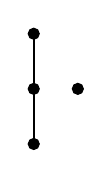
\begin{tikzpicture}[scale=.7,baseline=-5]
\draw[fill] (0,1) circle (1mm); 
\draw[fill] (0,0) circle (1mm); 
\draw[fill] (0,-1) circle (1mm); 
\draw[fill] (.8,0) circle (1mm); 
\draw[-,thick] (0,1) -- (0,0);
\draw[-,thick] (0,0) -- (0,-1);
\end{tikzpicture}\, ,
  \qquad
  (\mathbf2 + \mathbf2) =\,
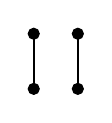
\begin{tikzpicture}[scale=.7,baseline=-5]
\draw[fill] (0,.5) circle (1mm); 
\draw[fill] (0,-.5) circle (1mm); 
\draw[fill] (.8,.5) circle (1mm); 
\draw[fill] (.8,-.5) circle (1mm); 
\draw[-,thick] (0,.5) -- (0,-.5);
\draw[-,thick] (.8,.5) -- (.8,-.5);
\end{tikzpicture}\,.
\end{equation*}
%For positive integers $a$, $b$, call a poset
%($\mathbf{a}+\mathbf{b}$)-{\em free}
%if it has no induced subposet isomorphic to a disjoint sum of an $a$-element
%chain and a $b$-element chain,
%and call the poset a {\em unit interval order} if it is
%($\mathbf{3}+\mathbf{1}$)-free
For example,
the
following
unit interval order
%poset
%$P$
%is a unit interval order
%($\mathbf3 + \mathbf 1)$-free and
%($\mathbf2 + \mathbf 2)$-free,
and
%has
%incomparability
graph
%$\inc(P) = G$.
\begin{equation}\label{eq:n+1}
  P = \ntnsp
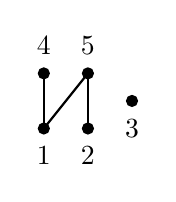
\begin{tikzpicture}[scale=.7,baseline=-5]
\draw[fill] (0,.5) circle (1mm); \node at (0,1) {$4$};
\draw[fill] (0,-.5) circle (1mm); \node at (0,-1) {$1$};
\draw[fill] (.8,.5) circle (1mm); \node at (.8,1) {$5$};
\draw[fill] (.8,-.5) circle (1mm); \node at (.8,-1) {$2$};
\draw[fill] (1.6,0) circle (1mm); \node at (1.6,-.5) {$3$};
\draw[-,thick] (0,.5) -- (0,-.5);%41
\draw[-,thick] (.8,.5) -- (0,-.5);%51
\draw[-,thick] (.8,.5) -- (.8,-.5);%52
\end{tikzpicture}\,,
\qquad \qquad
%\qquad 
  G = \ntnsp
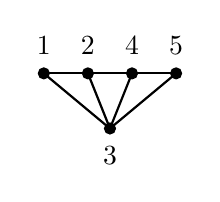
\begin{tikzpicture}[scale=.7,baseline=-5]
\draw[fill] (-1.2,.5) circle (1mm); \node at (-1.2,1) {$1$};
\draw[fill] (-.4,.5) circle (1mm); \node at (-.4,1) {$2$};
\draw[fill] (.4,.5) circle (1mm); \node at (.4,1) {$4$};
\draw[fill] (0,-.5) circle (1mm); \node at (0,-1) {$3$};
\draw[fill] (1.2,.5) circle (1mm); \node at (1.2,1) {$5$};
\draw[-,thick] (-1.2,.5) -- (0,-.5);%13
\draw[-,thick] (-.4,.5) -- (0,-.5);%23
\draw[-,thick] (.4,.5) -- (0,-.5);%43
\draw[-,thick] (1.2,.5) -- (0,-.5);%53
\draw[-,thick] (-1.2,.5) -- (-.4,.5);%12
\draw[-,thick] (-.4,.5) -- (.4,.5);%24
\draw[-,thick] (.4,.5) -- (1.2,.5);%45
\end{tikzpicture}\,
\end{equation}
satisfy $\inc(P) = G$.

%$\star$ Define altitude respecting labeling?  Or give 
%We remark that
%If we cannot interpret $\theta(\inc(P))$ for {\em all} posets $P$, sometimes
%we can do so when $P$ is ($\mathbf3 + \mathbf 1)$-free.
Given an $n$-element unit interval order $P$,
%poset $P$ which is
%a {\em unit interval order},
it is easy to explicitly describe
%to find
%a simple procedure produces
an element $D = D(P) \in \sn$
%$w \in \sn$
satisfying $Y(D) = X_{\inc(P)}$~\cite[\S 3]{SkanCCS}.  
\begin{alg}\label{a:PtoC}
  Given unit interval order $P$, do
  \begin{enumerate}
  \item For each element $y \in P$, compute
%\begin{equation*}%\label{eq:altitude}
$\beta(y) \defeq
  \# \{ x \in P \,|\, x \leq_P y \} - \# \{ z \in P \,|\, z \geq_P y \}.$
%\end{equation*}
  %and
  \item Label the poset elements $1, \dotsc, n$
so that we have
%$\beta(1), \dotsc, \beta(n)$ weakly increase.
%\begin{equation}\label{eq:altrespect}
  $\beta(1) \leq \cdots \leq \beta(n)$.
%  \end{equation}
%Then
\item Define $w = w(P) = w_1 \cdots w_n$ by
%\begin{equation}\label{eq:uioto312avoid}
  $w_j = \max ( \{ i \,|\, i \not >_P j \} \ssm \{ w_1, \dotsc, w_{j-1} \} )$.
  %\end{equation}
\item Define $D = \sum_{v \leq w} v$, where $\leq$ is the Bruhat order on $\sn$.
\end{enumerate}
\end{alg}
\noindent
The element $D$ produced by Algorithm~\ref{a:PtoC} is usually written
$C'_w(1)$ and is called the {\em Kazhdan--Lusztig basis element}
indexed by $w$~\cite{KLRepCH}.  (See \cite{BBCoxeter} for more
information on this basis and the Bruhat order.)
%It is known that $C'_w(1) = \sum_{v \leq w} w$.
%and define $D = D(w)
The map $P \mapsto w(P)$ defined by Steps 1--3 of Algorithm~\ref{a:PtoC}
is a bijection from $n$-element unit interval orders to the
%are in bijective correspondence with the
$\tfrac{1}{n+1}\tbinom{2n}n$ $312$-avoiding permutations in $\sn$,
%which avoid the pattern $312$.  To make this bijection explicit,
%we
%This bijection
and gives us the following result~\cite[Cor.\,7.5]{CHSSkanEKL}.
(See \cite{BilleyLak} for more information on pattern avoidance.)
\begin{prop}\label{p:uioto312avoid}
  Let $P$ be an $n$-element unit interval order and $w = w(P)$ be the
  corresponding $312$-avoiding permutation in $\sn$.  Then we have
  $Y(C'_w(1)) = X_{\inc(P)}$.
\end{prop}

For example, elements of the poset $P$ in (\ref{eq:n+1}) are already labeled
as in Step 2 of Algorithm~\ref{a:PtoC}:
%to satsify (\ref{eq:altrespect}),
%\begin{equation*}
%  \beta(1) = -2 < \beta(2) = -1 < \beta(3) = 0 < \beta(4) = 1 < \beta(5) = .2
  $(\beta(1), \beta(2), \beta(3), \beta(4), \beta(5)) = (-2, -1, 0, 1, 2)$.
%\end{equation*}
Thus we compute
\begin{equation*}
  w(P) = 34521,
  \qquad D = C'_{34521}(1) = \nTksp \sum_{v \leq 34521} \nTksp v,
  \end{equation*}
and we have $Y(C'_{34521}(1)) = X_{\inc(P)}$.
%The labeling (\ref{eq:altrespect}) of $P$ is {\em natural} in the sense that
%elements labeled $x$, $y$ satisfy
%\begin{equation}\label{eq:natlabel}
%  x <_P y \quad \Longrightarrow \quad x < y \text{ (as integers).}
%\end{equation}

%We remark that
The labeling in Step 2 of
Algorithm~\ref{a:PtoC}~\cite[p.\,33]{Fish}, \cite[\S 8.2]{Trott}
also associates a totally nonnegative matrix to a
unit interval order $P$.
%($\star$ Cite Fishburn and/or Trotter.)
Define the {\em antiadjacency matrix} of a labeled poset $P$ to be the matrix
$A = (a_{i,j})$ with entries
\begin{equation}\label{eq:antiadj}
  a_{i,j} = \begin{cases}
    0 &\text{if $i <_P j$},\\
    1 &\text{otherwise}.
  \end{cases}
\end{equation}
\begin{prop}
  For $P$ a unit interval order labeled as in
  %Step 2 of
  Algorithm~\ref{a:PtoC},
  the antiadjacency matrix $A = A(P)$ is totally nonnegative.
\end{prop}
\begin{proof}
%  The matrix $A$ is the transpose of a submatrix of the infinite
  %  Toeplitz matrix $B = (b_{i,j})$ defined by
  Entries of $A$ equal to $0$ form a Ferrers diagram in the upper right
  of the matrix.  Thus each submatrix of $A$
  has repeated rows and columns, or is unitriangular.
\end{proof}
%($\star$ Which of the following definitions related to poset tableaux are necessary?)

Combinatorial interpretations of numbers $\theta(\inc(P))$ often
involve generalizations of Young tableaux
%structures
called $P$-tableaux, and statistics on these.
Define a {\em $P$-tableau of shape $\lambda \vdash |P|$} to be
a filling of a
%(French)
Young diagram of shape $\lambda$ with the
elements of $P$, one per box.
%If $P$-tableau $U$ consists of a single row,
%we will call it a {\em $P$-permutation}.
%In particular, each concatenation $U_{i_1} \circ \cdots \circ U_{i_k}$
%of the rows (in any order) of a $P$-tableau $U$ is a $P$-permutation.
%If the elements of a poset are $[n] \defeq \{1, \dotsc, n\}$,
%We will sometimes write a $P$-tableau of shape $n$
%as an ordinary permutation
%$v_1 \cdots v_n \in \sn$. ($\star$ Do we actually do this?)
For example we have the poset $P$ and $P$-tableaux
\begin{equation}\label{eq:tableauxposet}
  P =
%\begin{equation*}%line 1
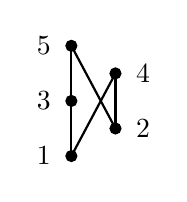
\begin{tikzpicture}[scale=.7,baseline=-5]
\draw[fill] (0,1) circle (1mm); \node at (-.5,1) {$5$};
\draw[fill] (0,0) circle (1mm); \node at (-.5,0) {$3$};
\draw[fill] (0,-1) circle (1mm); \node at (-.5,-1) {$1$};
\draw[fill] (.8,.5) circle (1mm); \node at (1.3,.5) {$4$};
\draw[fill] (.8,-.5) circle (1mm); \node at (1.3,-.5) {$2$};
\draw[-,thick] (0,1) -- (0,0);%53
\draw[-,thick] (0,0) -- (0,-1);%31
\draw[-,thick] (0,1) -- (.8,-.5);%52
\draw[-,thick] (0,-1) -- (.8,.5);%14
\draw[-,thick] (.8,.5) -- (.8,-.5);%42
\end{tikzpicture},
\qquad \qquad%
\begin{gathered}
  T \ntnsp= {\tableau[scY]{5|2,4|1,3}}\,, \quad 
  U = {\tableau[scY]{5,4|1,2,3}}\,, \quad
  V \ntnsp= {\tableau[scY]{5,4|3,1,2}}\,, \\
%  \begin{gathered}
%    W = {\tableau[scY]{5,4,1,2,3}}\,, \qquad
%    W = {\tableau[scY]{5,4,1,2,3}}\,,
%  \end{gathered}
%  \begin{gathered}
  \phantom{\sum^\sum} \nTksp
  W = {\tableau[scY]{5,4,1,2,3}}\,.
  %\quad
%%&= 54123%\phantom{\int}
%W' = {\tableau[scY]{1,2,3,5,4}}\,,
%\end{gathered}  
%\qquad \,
%\begin{gathered}
%  U = {\tableau[scY]{4,5|1,3,2}}\,\raisebox{-4mm},\\
%\underset{\phantom m}{U_2} = {\tableau[scY]{5,4}}\,,\\
%U_{2,1} = 5,%\phantom{\int}
\end{gathered}
%\qquad \,
%\begin{aligned}
%\underset{\phantom m}{W} &= {\tableau[scY]{5,4,1,2,3}}\,,\\
%&= 54123%\phantom{\int}
%\underset{\phantom m}{W'} &= {\tableau[scY]{1,2,3,5,4}}\,,\\
%\end{aligned}
\end{equation}
%\begin{equation}\label{eq:tabx}
%  \,
%  T \ntnsp= {\tableau[scY]{5|2,4|1,3}}\,,\ \,
%%  \quad
%  U \ntnsp= {\tableau[scY]{5,4|1,2,3}}\,,\ \,
%%  \quad
%  V \ntnsp= {\tableau[scY]{4,5|1,3,2}}\,,\ \,
%%  \quadd 
%  W \ntnsp= {\tableau[scY]{5,4|3,1,2}}\,,\ \,
%%  \quad
%  U_2 \circ U_1 \ntnsp= {\tableau[scY]{5,4,1,2,3}}\,.
%\end{equation}  
%of shapes $221$, $32$, and $5$,
%with $W$
%and $W'$
%essentially being the permutation
%$54123 \in \mfs 5$.
%, $12354$ in $\mfs 5$.
%($\star$ Remove $W$, $W'$? or maybe just $W'$? Or replace them
%with a tableau which is neither row-semistrict nor column-strict?)
%satisfy $\sh(T) = 221$.
%, (\ref{eq:tableauxposet}) shows
%a poset $P$,
%a $P$-tableau $T$ of shape $221$,
%two $P$-tableaux $U$, $V$ of shape $32$,
%and two $P$-tableaux $W$, $W'$ of shape $5$
%the second row $U_2$
%and entry $U_{2,1}$ of $U$, and the $P$-permutation $U_2 \circ U_1$
%which may be viewed as an element of $\mfs 5$.

The statistics we apply to $P$-tableaux are
%natural
$P$-analogs of traditional
permutation statistics.
Given a $P$-tableau $U$,
let $U_i$ be the $i$th row (from the bottom) of $U$,
and let $U_{i,j}$ be the $j$th entry in row $i$.
Call a position $(i,j)$ in $U$ a {\em descent}
%in $U$ to be a position $(i,j)$ such that
if $U_{i,j} >_P U_{i,j+1}$,
and a {\em record}
%in $U$ to be a position $(i,j)$ such that
if
%$j > 1$ and
$U_{i,1}, \dotsc, U_{i,j-1} <_P U_{i,j}$.
Define
%and define
%\begin{equation*}
%  \begin{aligned}
%\des_P(U) &=\, \text{number of descents in } U,\\
%\rec_P(U) &= \text{number of
%records in } U.
%  \end{aligned}
%\end{equation*}
%$\des_P(U) = \#$ descents in $U$;
%$\rec_P(U) = \#$ records in $U$,
$\des_P(U)$ and $\rec_P(U)$
%= \#$ descents in $U$;
to be the numbers of descents and records in $U$, respectively,
and call $U$
\begin{enumerate}
\item {\em descent-free} or {\em row-semistrict} if $\des_P(U) = 0$,
  %Call $U$
\item {\em column-strict} if the entries of each column satisfy
  $U_{i,j} <_P U_{i+1,j}$,
  %Call $U$
\item {\em standard} if it is column-strict and row-semistrict.
%    Call $U$
%\item ($\star$ remove?) {\em cyclically row-semistrict} if it is row-semistrict and if
%  $U_{i,\lambda_i} \not >_P U_{i,1}$ for all $i$,
%\item ($\star$ remove?) {\em $P$-excedance-free} if $\exc_P(U) = 0$,
%\item {\em record-free} if it has no nontrivial $P$-records.
\end{enumerate}
For example,
the tableaux in (\ref{eq:tableauxposet}) satisfy
%we look again at the poset $P$ in (\ref{eq:tableauxposet}),
%the $P$-tableaux there, and three more,
%$U_2 \circ U_1$
%and three more $P$-tableaux
%\begin{equation}\label{eq:tabx}
%  \,
%  T \ntnsp= {\tableau[scY]{5|2,4|1,3}}\,,\ \,
%%  \quad
%  U \ntnsp= {\tableau[scY]{5,4|1,2,3}}\,,\ \,
%%  \quad
%  V \ntnsp= {\tableau[scY]{4,5|1,3,2}}\,,\ \,
%%  \quad
%  W \ntnsp= {\tableau[scY]{5,4|3,1,2}}\,,\ \,
%%  \quad
%  U_2 \circ U_1 \ntnsp= {\tableau[scY]{5,4,1,2,3}}\,.
%\end{equation}  
%we have
$\des_P(T) = \des_P(U) 
% = \des_P(W')
= 0$,
%while
$\des_P(V) = \des_P(W) = 1$,
%because $3 >_P 1$ and $4 >_P 1$.
%We have that
and
$\rec_P(W) = 1$,
$\rec_P(U) = \rec_P(V)
%= \rec_P(W')
= 2$,
%are $P$-record-free,
%since the first entry in each row of these tableaux
%is greater than or incomparable to the remaining entries in the same row.
%On the other hand,
$\rec_P(T) = 5$.
%since $1 <_P 3$ and
%$2 <_P 4$.
%, and $\rec_P(W') = 1$ since $1, 2, 3 <_P 5$.
%Reordering the entries of each row in the tableaux above
%(\ref{eq:tabx})
%we obtain
%\begin{equation*}
%  \ol T = {\tableau[scY]{5|2,4|1,3}}\,,
%  \quad
%  \ol U = {\tableau[scY]{5,4|1,2,3}}\,,
%  \quad
%  \ol V = {\tableau[scY]{4,5|1,3,2}}\,,
%  \quad
%  \ol W = {\tableau[scY]{5,4|3,1,2}}\,,
%  \quad
%  \ol{U_2 \circ U_1} = {\tableau[scY]{5,4,1,2,3}}\,.
%\end{equation*}  
%or
%\begin{equation*}
%  %\label{eq:bartabx}
%  \ol T = T, \qquad
%  \ol U = \ol V = \ol W = {\tableau[scY]{4,5|1,2,3}}\,, \qquad
%  \ol{U_2 \circ U_1} = {\tableau[scY]{1,2,3,4,5}}\,.
%\end{equation*}
%Comparing
%the tableaux
%$T$, $U$, $V$ with $\ol T$, $\ol U$, $\ol V$,
%their reordered counterparts,
%we have $\exc_P(T) = \exc_P(U) = \exc_P(V) = 0$.
%Comparing $W$ and $\ol W$, we see that
%position $(1,1)$ is the only $P$-excedance:
%$3 >_P 1$. Thus $\exc_P(W) = 1$.
%Comparing $U_2 \circ U_1$ to $\ol{U_2 \circ U_1}$, we see that
%positions $(1,1)$ and $(1,2)$ are both $P$-excedances:
%and $\exc(U_2 \circ U_1) = 2$ since
%$5 >_P 1$, $4 >_P 2$.
%Thus $\exc_P(U_2 \circ U_1) = 2$.
Tableaux $T$, $U$, are row-semistrict,
%but not column-strict,
$U$, $V$, $W$ are column-strict, and
$U$ is standard.
%is but not
%Using comparability in $P$ and the above statistics,
%we define three
%four
%classes of $P$-tableaux.
%Call a $P$-tableau $U$ of shape $\lambda$
%We will sometimes refer to a $P$-tableau of shape $n$ as a
%{\em $P$-permutation}, and if its
%$\star$ Give some examples.
%For example, applyingThe following table shows which
%For example, we may examine 
%for these properties to obtain the table
%posess the above properties.
%apply to the tableaux (\ref{eq:tabx}).
%which of the above properties.

%\vspace{2mm}
%\hhhsp
%\begin{center}
%\newcolumntype{R}{>{$}c<{$}}
%\begin{tabularx}{122.9mm}{|R|R|R|R|R|R|}%
%\hline
%\phsum & \phm T\phm & \phm U\phm & \phm V\phm & \phn W\phn & \phn W'\phn \\
%\hline 
%\phsum\mbox{row-semistrict}\phsum
%& \checkmark & \checkmark &            &            & \checkmark \\
%\phsum\mbox{column-strict}\phsum
%&            & \checkmark & \checkmark & \checkmark & \checkmark \\
%\phsum\mbox{standard}\phsum
%&            & \checkmark &            &            & \checkmark \\
%\hline
%\end{tabularx}\,.
%\end{center}
%\vspace{3mm}
%\ssp

In terms of the above definitions, we have the following
combinatorial interpretations of trace evaluations.
Interpretations of induced sign character evaluations are
%perhaps
the simplest.  (See, e.g., \cite[Eqn.~(3.11)]{SkanCCS}.)
\begin{thm}\label{t:epsilonevals}
  Let $G$ be any (simple) graph on $n$ vertices,
  and let $P$ be any poset on $n$ elements.  For all $\lambda \vdash n$
  we have
  \begin{enumerate}
  \item $\epsilon^\lambda(G)$ is $c(G,\lambda)$, the number of
    proper colorings of $G$ of type $\lambda$.
  \item $\epsilon^\lambda(\inc(P))$ is the number of column-strict
    $P$-tableaux of shape $\lambda^\tr$.
  \end{enumerate}
\end{thm}
\noindent
Induced trivial character evaluations are also rather
simple~\cite[Thm.\,4.7 (ii-b)]{CHSSkanEKL}, \cite[Thm.\,3.7]{SkanCCS}.
\begin{thm}\label{t:etaevals}
  Let $G$ be any (simple) graph on $n$ vertices,
  and let $P$ be any poset on $n$ elements.
  For all $\lambda  = (\lambda_1,\dotsc, \lambda_r) \vdash n$
  we have
  \begin{enumerate}
  \item $\eta^\lambda(G)$ is the number of sequences $(O_1,\dotsc,O_r)$
    of acyclic orientations of
    %sequences $(G_1,\dotsc,G_r)$ of
    induced subgraphs
    %$G_i = (V_i, E_i)$
    of $G$ on pairwise disjoint vertex
    subsets of cardinalities $\lambda_1,\dotsc,\lambda_r$.
    %$(V_1,\dotsc, V_n)$ satisfying
    %$(|V_1|, \dotsc, |V_n|) = \lambda$.
%  \item $\eta^\lambda(G)$ is the number of pairs of sequences
%    $((G_1,\dotsc, G_r),(O_1,\dotsc,O_r))$
%    where $(G_1,\dotsc,G_r)$ are induced subgraphs
%    of $G = (V,E)$ on pairwise disjoint vertex
%    subsets $(V_1,\dotsc, V_n)$ satisfying
%    $(|V_1|, \dotsc, |V_n|) = \lambda$, and $(O_1,\dotsc,O_n)$
%    are acyclic orientations of these.
  \item $\eta^\lambda(\inc(P))$ is the number of row-semistrict
    $P$-tableaux of shape $\lambda$.
  \end{enumerate}
\end{thm}
\noindent 
%\ssec{Irreducible characters / Schur coefficients of $X_{\inc(P)}$}
While $\chi^\lambda(G)$ is negative for some graphs $G$,
even for some incomparability graphs $\inc(P)$,
%$\chi^\lambda(\inc(P))$ is negative for some posets $P$,
Stanley and Stembridge~\cite[Conj.\,5.1]{StanStemIJT}
conjectured $\chi^\lambda(\inc(P))$ to be nonnegative
for $(\mathbf3 + \mathbf 1)$-free posets $P$.
%($\star$ Define more properties?)
Gasharov~\cite{GashInc} proved this,
and Kaliszewski~\cite[Prop.\ 4.3]{KaliHook}
showed that when $\lambda$ is a hook partition,
the evaluation $\chi^\lambda(\inc(P))$
is nonnegative for all posets $P$.
Combining these results into one statement, we have the
following.
%is indeed positive for by
%showing that for these posets we have
%using standard $P$-tableaux.
%to prove the 
%($\star$ cite Stanley-Stembridge)
%nonnegativity of $\chi^\lambda(\inc(P))$
%For $P$ avoiding 
%(but not necessarily $\mathbf2 + \mathbf2$),
%one may use $P$-tableaux~\cite{GV} to state
%simple combinatorial interpretations of the coefficients which
%arise in the expansion of $X_{\inc(P)}$ in the
%monomial basis (by definition),
%and Schur basis (by the following result of Gasharov).
%yields coefficients
%$\{ \epsilon^\lambda(\wtc w1) \,|\, \lambda \vdash n \}$
%which are 
%For these posets and even the more general class of
%($\mathbf3 + \mathbf1$)-free posets, the expansions of functions
%$X_{\inc(P)}$ were
%conjectured coefficients of the Schur expansions
%of
%$X_{\inc(P)}$ in different symmetric
%have combinatorial interpretations which may be
%simply stated in terms of $P$-tableaux~\cite{GV}. 
%we have the following result of Gasharov~\cite{GashInc},
%which settled the conjectured
%Schur-positivity~($\star$ Cite Stanley, Stembridge) of $X_{\inc(P)}$
%for ($\mathbf3 + \mathbf1$)-free posets,
%originally conjectured in~\cite{StanStemIJT}.
%with the following result.
%\begin{prop}\label{p:Gash}
%  For $P$ a ($\mathbf3 + \mathbf1)$-free poset,
  %each number
\begin{thm}\label{t:KaliGash}
  Let $P$ be an $n$-element poset.
  \begin{enumerate}
  \item For $\lambda \vdash n$ a hook shape,
    %then
      $\chi^\lambda(\inc(P))$ is the number of
      standard $P$-tableaux of shape $\lambda$.
  \item %For $\lambda \vdash n$ arbitrary and 
      If $P$ is $(\mathbf3+\mathbf1$)-free then for any
      $\lambda \vdash n$,
      $\chi^\lambda(\inc(P))$ is the number of
      standard $P$-tableaux of shape $\lambda$.
  \end{enumerate}
  \end{thm}
    
%  \begin{equation}\label{eq:Gash}
%  \chi^\lambda(\inc(P)) = 
  %and choose $g \in \qsn$
  %such that $Y_q(g) = X_{\inc(P)}$.  Then for all $\lambda \vdash n$,
  %the evaluation $\chi^\lambda(g)$
  %(equivalently, the coefficient of $s_{\lambda^\tr}$ in $X_P$
  %and the coefficient of $s_\lambda$ in $\omega X_P$)
  %is equal to
%  \# \text{ standard $P$-tableaux of shape $\lambda$}.
%  \end{equation}
%\end{prop}
%Using Chow's statment 
%Kaliszewski~\cite[Prop.\ 4.3]{KaliHook} extended this result to
%all posets $P$ 
%that
%when $\lambda$ is a hook shape.

%A consequence of Kaliszewski's
%result~\cite[Prop.\ 4.3]{KaliHook} is the following.
%The above bijections relate
%column-strict $P$-tableaux of arbitrary shape
%to standard $P$-tableaux of hook shape. 
%The above bijections relate standard $P$-tableaux
%to column-strict $P$-tableaux.
%$\star$ Now introduce this proposition and shorten its proof.
%\begin{prop}\label{p:Kali}
%  For any $n$-element poset $P$ and hook shape
  %be any poset and choose $g \in \qsn$
  %such that $Y_q(g) = X_{\inc(P)}$.  Then for the hook shape
%  $k1^{n-k} \vdash n$,
%  the evaluation
%  $\chi^{\smash{k1^{n-k}}}(\inc(P))$
  %(equivalently, the coefficient of $s_{(n-k+1)1^{k-1}}$ in $X_P$
  %and the coefficient of $s_{k1^{n-k}}$ in $\omega X_P$) 
%  (equivalently, the coefficient of $s_{\lambda^\tr}$ in $X_P$
%  and the coefficient of $s_\lambda$ in $\omega X_P$)
%  is the number of standard $P$-tableaux of shape $\lambda$.
%\
%For any poset $P$,
%equals the number of standard $P$-tableaux of shape $k1^{n-k}$.
%\end{prop}

%\begin{cor}\label{c:binom}
%  If $P$ is an $n$-element chain, then
%  $\chi^{k1^{n-k}}(\inc(P)) = \tbinom{n-1}{k-1}$.
%\end{cor}
%\begin{proof}
%Element $1$ must be placed in position (1,1),
%$k-1$ other elements must be chosen and placed uniquely
%in increasing order in column $1$,
%the remaining $n-k+1$ elements are placed uniquely
%in increasing order in row $1$.
%\end{proof}
%($\star$ Omit the above?  This is the same as the proof of Observation~\ref{o:hookchie}.)

%($\star$ Below, $P$ should really by $\inc(P)$.)
Observation~\ref{o:hookchie} and Theorem~\ref{t:KaliGash}
%this result
imply
%follows
that when $P$ is an $n$-element chain, the hook irreducible
character evaluations
%$\chi^n(\inc(P)), \chi^{n-1,1}(\inc(P)), \chi^{n-2,1^2}(\inc(P)), \dotsc, \chi^{1^n}(\inc(P))$
$\chi^{k1^{n-k}}(\inc(P)) = \tbinom{n-1}{k-1}$
and $\chi^{(k-1)1^{n-k+1}}(\inc(P)) = \tbinom{n-1}{k-2}$
are related by
\begin{equation}\label{eq:hookchareqs}
  (k-1) \chi^{k1^{n-k}}(\inc(P)) = (n-k+1) \chi^{k-1,1^{n-k+1}}(\inc(P))
\end{equation}
for $k = 2,\dotsc,n$.
For an arbitrary poset $P$ no analogous equality
%as simple as that of Corollary~\ref{c:binom}
exists, but we do have similar
%Nevertheless, we have
inequalities.
%analogous to (\ref{eq:hookchareqs}).
%no such simple formula exists.
%On the other hand, we can relate the values of
%$\chi^{k1^{n-k}}(\inc(P))$
%and
%$\chi^{(k-1)1^{n-k+1}}(\inc(P))$ as follows.
\begin{lem}\label{l:hookineq}
  For each naturally labeled $n$-element poset $P$ and $k = 2,\dotsc,n$
  we have
  %and define $d_i$ to be the number of
  %standard $P$-tableaux of shape $i1^{n-i}$.
  %Then we have $(k-1)d_k \geq (n-k+1)d_{k-1}$.
  \begin{equation}\label{eq:binomapprox}
    (k-1) \chi^{k1^{n-k}}(\inc(P)) \geq (n-k+1) \chi^{k-1,1^{n-k+1}}(\inc(P)).
  \end{equation}
  Furthermore, the difference
%  $(k-1)d_k - (n-k+1)d_{k-1}$
   $(k-1) \chi^{k1^{n-k}}(\inc(P)) - (n-k+1) \chi^{k-1,1^{n-k+1}}(\inc(P))$
  equals the number of standard $P$-tableaux
  of shape $k1^{n-k}$ in which one entry of the first row is marked
  and is incomparable in $P$ to an entry in an earlier column of the tableau.
  %satisfies at least one of the conditions
  %\begin{enumerate}
  %\item $j$ for all $i$ to the left of $j$ in row $1$,
  %  \item $i$ is 
\end{lem}
\begin{proof}
  Let $\mathcal C_k = \mathcal C_k(P)$
  be the set of standard $P$-tableaux of shape
  $k 1^{n-k}$ in which one entry of column $1$
  other than that in position $(1,1)$ is marked.
  Let $\mathcal R_k = \mathcal R_k(P)$
  be the set of standard $P$-tableaux of shape
  $k 1^{n-k}$ in which one entry of row $1$
  other than that in position $(1,1)$ is marked.
  The inequality (\ref{eq:binomapprox}) asserts that
  $|\mathcal R_k| \geq |\mathcal C_{k-1}|$.
  To see this, we define a family of maps
  $\{f_k: \mathcal C_{k-1} \rightarrow \mathcal R_k \,|\, k = 2,\dotsc, n\}$,
  by letting
  $f_k(U)$ be the tableau constructed from $U$ by
  removing the marked element from the first column of $U$,
  and reinserting it as far as possible to the right in row $1$
  subject to the requirement that it be a record.
  %o that it is a record.

  To see that the map $f_k$ is well-defined,
  let $m \in [n]$ be the marked element in column $1$ of $U$.
  Since $U$ is standard,
  $m$ must be greater than the element in position $(1,1)$.
  Thus it will certainly be inserted into positions $(1,2), \dotsc, (1,k-1)$
  or at the end of row $1$, creating a tableau of shape $k1^{n-k}$ with
  one marked element in the first row.
  We claim that the map $f_k$ is injective.
  To see this,
  %that it is injective,
  consider a tableau $V \in \mathcal R_{k}$
  which satisfies $V = f_k(U)$ for some $U \in \mathcal C_{k-1}$.
  A marked element $i$ in row $1$ of $V$ will necessarily be greater in $P$
  than all elements to its left in row $1$, and will be comparable in $P$
  to all elements in column $1$.
  To recover $U$, remove $i$ from row $1$ of $V$
  and insert it into the unique position of column $1$ so that entries there
  increase.  The resulting tableau will still be $P$-semistrict
  because if the element preceding $i$ in $V$, say $h$,
  and the element following $i$ in $V$, say $j$,
  satisfy $h >_P j$, then we have $i >_P h >_P j$, contradicting
  the semistrictness of row $1$ of $V$.
  
  To see that the difference
%  $(k-1)d_k - (n-k+1)d_{k-1}$
  $(k-1) \chi^{k1^{n-k}}(P) - (n-k+1) \chi^{k-1,1^{n-k+1}}(P)$
  has the claimed interpretation, consider the
  elements of $\mathcal R_k \ssm f(C_{k-1})$.
  These are standard $P$-tableaux $V$
  which contain a marked element $i$ in row $1$
  which is not a record in row $1$, or which is incomparable to
  some element of column $1$.  We claim that if $i$ is
  %comparable to all elements of column $1$ and
  not a record in row $1$, then it must
  be incomparable to an element to its left in row $1$.
  Assume otherwise: assume that $i$ follows $h$ in row $1$ with $h <_P i$
  and that some element $j >_P i$ appears earlier than $h$ in row $1$.
  Assume that $j$ is the rightmost such element with these properties.
  Then we have $j >_P h$.
  Let $g$ be the element immediately following $j$ in row $1$.
  By our choice of $j$ we cannot have $g >_P j$,
  and since $V$ is standard we cannot have $j >_P g$.
  Thus $j$ must be incomparable to $g$.
  %we cannot have $j <_P g$ or $g >_P i$.
  %Since $V$ is standard, we cannot have $j >_P g$.
  By our choice of $j$ we cannot have $g >_P i$,
  and our assumption on $i$ we cannot have $g$ incomparable to $i$.
  Thus we have $g <_P i$.  But then we have $g <_P i <_P j$, a contradiction.
\end{proof}
For example, define $\mathcal C_k$ and $\mathcal R_k$ as in the proof
of \ref{l:hookineq}, and consider
the poset $P$ in (\ref{eq:tableauxposet}).
The set $\mathcal C_3$
%defined in the proof of \ref{l:hookineq}
consists of two tableaux.  Applying $f_4$ to these we have
\begin{equation*}
  f_4\ntksp\left( \;\tableau[scY]{5|\circd3|1,2,4}\; \right) =
  \;\tableau[scY]{5|1,\circd3,2,4}\,, \qquad
  f_4\ntksp\left( \;\tableau[scY]{\circd 5|3|1,2,4}\; \right) =
  \;\tableau[scY]{3|1,2,\circd5,4}\,,
\end{equation*}
and the difference
$3 \chi^{41}(P) - 2 \chi^{311}(P)$ counts elements of $\mathcal R_4$
whose first row contains a marked element which is not a record
in that row, or which is incomparable to some element of the first column,
\begin{equation*}
  \;\tableau[scY]{5|1,3,\circd2,4}\,, \qquad
  \;\tableau[scY]{5|1,3,2,\circd4}\,, \qquad
  \;\tableau[scY]{5|1,\circd4,3,2}\,, \qquad
  \;\tableau[scY]{5|1,4,\circd3,2}\,, \qquad
  \;\tableau[scY]{5|1,4,3,\circd2}\,, \dotsc.
  \end{equation*}
%($\star$ Do an example to make the lemma and proof come
%alive.)

The statement preceding Theorem~\ref{t:KaliGash} implies
that $\phi^\lambda(G)$ is negative for some graphs $G$,
even for some incomparability graphs $G = \inc(P)$.
Hikita~\cite[Thm.\,3]{HikitaProof} showed that it is positive
for $G = \inc(P)$ and $P$ a $(\mathbf3 + \mathbf1)$-free poset,
%$P$,
settling the Stanley--Stembridge conjecture~\cite[Conj.\,5.5]{StanStemIJT}.
\begin{thm}\label{t:hikita}
  For $P$ a $(\mathbf3 + \mathbf1)$-free poset
  and $\lambda \vdash n$,
  we have $\phi^\lambda(\inc(P)) \geq 0$.
\end{thm}

\noindent
Hikita's proof unfortunately
does not provide a combinatorial interpretation
of $\phi^\lambda(\inc(P))$.
\bp
Find a combinatorial interpretation for 
$\phi^\lambda(\inc(P))$ which holds for all $\lambda \vdash n$ and for
$n$-element posets $P$ avoiding $\mathbf3 + \mathbf1$.
%and 
\ep

A related result for
monomial traces~\cite[Lem.\,4.1]{AthanPSE}, \cite[Thm.\,3.3]{StanSymm}
concerns sums
%of monomial traces
of the form
%s
  \begin{equation}\label{eq:thetaldef}
    \theta^\ell = \sumsb{\mu \vdash n\\\ell(\mu) = \ell} \ntnsp \phi^\mu.
  \end{equation}
%with $1 \leq \ell \leq n$.
\begin{prop}\label{p:stanksources}
  Let $G$ be any (simple) graph on $n$ vertices,
  and let $P$ be any poset on $n$ elements.
  The traces $\{ \theta^\ell \,|\, 1 \leq \ell \leq n \}$
  satisfy
%  and define the traces $\theta^1,\dotsc,\theta^n$ by
%  we have 
%  \begin{equation*}
%    \sumsb{\lambda\vdash n\\ \ell(\lambda) = k} \phi^\lambda(G)
  \begin{enumerate}
  \item $\theta^\ell(G)$ is the number of acyclic
    orientations of $G$ having $\ell$ sources,
    \item
      $\theta^\ell(\inc(P))$ is the number of
      descent-free $P$-tableaux of shape $n$ having $\ell$
      records.
      %permutations $w \in \sn$ satisfying
      %$\des_P(w) = 0$, $\rec_P(w) = \ell$.
  \end{enumerate}
\end{prop}

%\end{equation*}
%and for all $n$-element posets $P$ we have
%  \begin{equation*}
%    \sumsb{\lambda\vdash n\\ \ell(\lambda) = k} \phi^\lambda(\inc(P))
%    = \# \text{ $P$-descent-free $P$-permutations with $k$ $P$-records}.
%  \end{equation*}
%\end{prop}

%\begin{prop}\label{p:thetak}
%  Define traces $\theta^1,\dotsc, \theta^n$ by
%  \begin{equation*}
%    \theta^k = \sumsb{\lambda \vdash n\\\ell(\lambda) = k} \phi^\lambda,
%  \end{equation*}
%  and let $n \times n$ matrix $A$ be the path matrix of
%  planar network $F$.
%  Then we have
%  \begin{equation*}
%    \imm{\theta^k}(A) = \text{\# row-semistrict $F$-tableaux with $k$ records}.
%    \end{equation*}
%\end{prop}

\section{Applications to total nonnegativity}\label{s:tnn}

Nonnegative expansions of chromatic symmetric functions in
the standard bases
%various symmetric function bases
are closely
related to
the immanants defined in (\ref{eq:immdef})
and to certain directed planar graphs.
%called {\em planar networks}.
%certain
%functions of totally nonnegative matrices,
%defined in Section~\ref{s:intro}.
We will make these relationships precise in Proposition~\ref{p:immincP}
and state some immanantal analogs of results from Section~\ref{s:chrom}.
%($\star$ Also summarize the remainder of the section.)
%y~\ref{c:tnnimplications}.
%Call a real $n \times n$ matrix $A = (a_{i,j})$ {\em totally nonnegative} if
%for each pair $(I,J)$ of subsets of $[n]$,
%$ \defeq \{1,\dotsc,n\}$,
%the square submatrix $A_{I,J} \defeq (a_{i,j})_{i\in I, j\in J}$
%satisfies $\det(A_{I,J}) \geq 0$. 
%Such matrices are closely related to directed graphs called planar networks.

Define a (nonnegative weighted)
{\em planar network of order $n$} to be a directed, planar, acyclic
digraph $F = (V,E)$
which can be embedded in a disc so that $2n$ distinguished vertices
labeled clockwise as $s_1,\dotsc,s_n,t_n,\dotsc,t_1$
lie on the boundary of the disc,
with a nonnegative real {\em weight} $c_{u,v}$
%$\in \mathbb R_{\geq 0}$
assigned to each edge $(u,v) \in E$.
We may assume that $s_1,\dotsc,s_n$, called {\em sources}, have indegree $0$
and that $t_n,\dotsc,t_1$, called {\em sinks}, have outdegree $0$.
To every source-to-sink path, we associate a weight equal to the product
of its edge weights,
%of its edges,
and we define the {\em path matrix}
$A = A(F) = (a_{i,j})_{i,j \in [n]}$ by
%\begin{equation*}
setting $a_{i,j}$ equal to the sum of weights of all paths
%$s_i$-to-$t_j$ paths.
from $s_i$ to $t_j$.
For example, one
%we have the following
planar network $F$ of order $3$, with edges weighted by positive numbers
$1, a, \dotsc, h$,
and its path matrix $A$ are
%($\star$ Omit vertex labels $v_1,\dotsc,v_4$ below?)
%($\star$ recompute $A$)
%in which
%Unlabeled edges have weight $1$.

\begin{equation}\label{eq:planarnet}
    F = \ntnsp
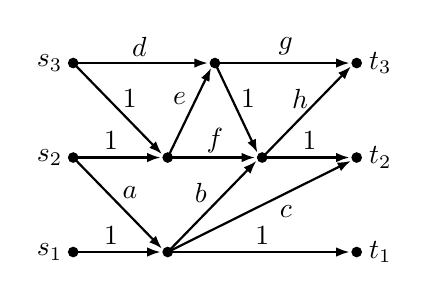
\begin{tikzpicture}[scale=.6,baseline=-5]
\draw[fill] (0,2) circle (1mm); \node at (-.5,2) {$s_3$};
\draw[fill] (0,0) circle (1mm); \node at (-.5,0) {$s_2$};
\draw[fill] (0,-2) circle (1mm); \node at (-.5,-2) {$s_1$};
\draw[fill] (3,2) circle (1mm); %\node at (3.1,2.35) {$v_3$};
\draw[fill] (2,0) circle (1mm); %\node at (2,-.35) {$v_2$};
\draw[fill] (2,-2) circle (1mm); %\node at (2,-2.35) {$v_1$};
\draw[fill] (4,0) circle (1mm); %\node at (4.15,-0.35) {$v_4$};
\draw[fill] (6,2) circle (1mm); \node at (6.5,2) {$t_3$};
\draw[fill] (6,0) circle (1mm); \node at (6.5,0) {$t_2$};
\draw[fill] (6,-2) circle (1mm); \node at (6.5,-2) {$t_1$};
\node at (.8,.35) {$1$};
\node at (.8,-1.65) {$1$};
\node at (1.2,1.25) {$1$};
\node at (1.2,-.75) {$a$};
\node at (1.4,2.35) {$d$};
\node at (2.25,1.25) {$e$};
\node at (2.7,-.75) {$b$};
\node at (3,.35) {$f$};
\node at (3.7,1.25) {$1$};
\node at (4,-1.65) {$1$};
\node at (4.5,2.35) {$g$};
\node at (4.5,-1.15) {$c$};
\node at (4.8,1.25) {$h$};
\node at (5,.35) {$1$};
\draw[->,thick] (0,2) -- (2.85,2);%s3v3
\draw[->,thick] (0,2) -- (1.88,0.07);%s3v2
\draw[->,thick] (0,0) -- (1.85,0);%s2v2
\draw[->,thick] (0,0) -- (1.88,-1.93);%s2v1
\draw[->,thick] (0,-2) -- (1.85,-2);%s1v1
\draw[->,thick] (2,0) -- (2.92,1.9);%v2v3
\draw[->,thick] (2,0) -- (3.85,0);%v2v4
\draw[->,thick] (2,-2) -- (3.88,-.07);%v1v4
\draw[->,thick] (2,-2) -- (5.88,-.07);%v1t2
\draw[->,thick] (2,-2) -- (5.85,-2);%v1t1
\draw[->,thick] (3,2) -- (5.85,2);%v3t3
\draw[->,thick] (3,2) -- (3.9,.1);%v3v4
\draw[->,thick] (4,0) -- (5.88,1.93);%v4t3
\draw[->,thick] (4,0) -- (5.85,0);%v4t2
%\draw[<-,thick] (-.35,.35) -- (0,-.5);%23
%\draw[->,thick] (.4,.5) -- (0.05,-.35);%43
%\draw[<-,thick] (-.25,.5) -- (.4,.5);%24
%\draw[->,thick] (-.4,.5) -- (.25,.5);%24
%\draw[-,thick] (-.4,.5) -- (0,-.5);%23
%\draw[-,thick] (.4,.5) -- (0,-.5);%43
%\draw[-,thick] (-.4,.5) -- (.4,.5);%24
\end{tikzpicture}\ntnsp,
\qquad
A = \begin{bmatrix}
  1 & b+c & \ntnsp bh \\
  a & ab\ntnsp+{\ntnsp}ac\ntnsp+{\ntnsp}e\ntnsp+{\ntnsp}f & \ntnsp abh+fh+eh+eg \\
  0 & e+f & \ntnsp dh\ntnsp+\ntnsp eh\ntnsp+\ntnsp fh\ntnsp+\ntnsp eg\ntnsp+\ntnsp dg
\end{bmatrix}\ntksp.\nTksp
%\draw[fill] (1,1) circle (1mm); \node at (1,-.5) {$x$};
\end{equation}

A result often attributed to Lindstr\"om
~\cite{LinVrep} but proved earlier by Karlin and McGregor~\cite{KMG}
asserts the total nonnegativity of such a matrix.
%\begin{thm}\label{t:lin}
%  The path matrix $A$ of a nonnegative weighted planar network $G$ of order $n$
%  is totally nonnegative.  Moreover, for each pair
%  $I = \{ i_1, \dotsc, i_d \}, J = \{ j_1,\dotsc,j_d\} \subseteq [n]$, 
%  the nonnegative number $\det(A_{I,J})$ equals
%  \begin{equation*}
%    \prod_{\pi = (\pi_1,\dotsc,\pi_d)} \wgt(\pi_1) \cdots \wgt(\pi_d),
%  \end{equation*}
%  where the sum is over all families of pairwise nonintersecting paths
%  from $s_{i_1},\dotsc,s_{i_d}$ to $t_{i_1},\dotsc,t_{i_d}$.
%\end{thm}
\begin{thm}\label{t:lin}
  The path matrix $A$ of a nonnegative weighted planar network $F$ of order $n$
  is totally nonnegative.  Moreover,
  %for each pair
  %$I = \{ i_1, \dotsc, i_d \}, J = \{ j_1,\dotsc,j_d\} \subseteq [n]$, 
  the nonnegative number $\det(A)$ equals
  \begin{equation*}
%    \prod_{\pi = (\pi_1,\dotsc,\pi_n)} \wgt(\pi),
    \sum_\pi \wgt(\pi),
    %\cdots \wgt(\pi_n),
  \end{equation*}
  where the sum is over all families $\pi = (\pi_1,\dotsc,\pi_n)$
  of pairwise nonintersecting paths in $F$,
  with $\pi_i$ a path from $s_i$ to $t_i$ for $i = 1,\dotsc,n$, and where
  \begin{equation}\label{eq:wgt}
    \wgt(\pi) \defeq \wgt(\pi_1) \cdots \wgt(\pi_n).
    \end{equation}
  %$s_{i_1},\dotsc,s_{i_d}$ to $t_{i_1},\dotsc,t_{i_d}$.
\end{thm}

%Since each submatrix of a totally nonnegative matrix is itself totally
%nonnegative, this result gives a combinatorial interpretation of
%the nonnegative numbers $\det(A_{I,J})$
%%, when $|I| = |J|$,
%as well:
%$\det(A_{I,J})$ is the sum of weights of all nonintersecting path families
%in $D$ from sources indexed by $I$ to sinks indexed by $J$
%(assuming $|I| = |J|$).
%For example, in (\ref{eq:planarnet}), we have $\det(A) = 30$,
%and the one nonintersecting path family in $D$
%from $\{s_1, s_2, s_3\}$ to $\{t_1, t_2, t_3 \}$
%%all sources to all sinks of
%%$D$
%has weight
%$(1\cdot 1)(1 \cdot 5 \cdot 1)(1 \cdot 6) = 30$.
%Also, we have $\det(A_{13,23}) = 136$ and the three nonintersecting path families
%from $\{s_1,s_3\}$ to $\{t_2, t_3\}$ have weights
%$(1 \cdot 7)(1 \cdot 5 \cdot 2)$,
%$(1 \cdot 7)(1 \cdot 6)$, and
%$(1 \cdot 4 \cdot 1)(1 \cdot 6)$, which sum to $136$.
\noindent
Thus by inspection of the network $F$ in (\ref{eq:planarnet}),
its path matrix $A$ satisfies $\det(A) = fdg$.

The converse of Theorem~\ref{t:lin} is true as well.
That is,
path matrices are essentially the only examples of totally nonnegative
matrices
~\cite{BrentiCTP}, \cite{CryerProp}, \cite{loewner}, \cite{WReduction}.
%By results of
%By results of Whitney
%Loewner
%Cryer
%and Brenti
%Loewner et.~al.~\cite{Loewner} ($\star$ cite others too)
%
\begin{thm}\label{t:tnnconv}
  For each $n \times n$ totally nonnegative matrix $A$, there exists
  a nonnegative weighted planar network of order $n$
  whose path matrix is $A$.
\end{thm}

Also belonging to the subject of total nonnegativity are polynomial functions
\begin{equation*}
  f(x)
  \defeq
  f(x_{1,1}, x_{1,2}, \dotsc, x_{n,n}) \in
  %\in
  %\mathbb Z[x] \defeq
  \mathbb Z[x_{1,1},x_{1,2},\dotsc,x_{n,n}]
  \end{equation*}
%that evaluate nonnegatively on totally nonnegative matrices,
%i.e.,
having the property that
%with the property that
\begin{equation*}
  f(A) \defeq f(a_{1,1},a_{1,2},\dotsc,a_{n,n}) \geq 0
\end{equation*}
for all totally nonnegative matrices $A = (a_{i,j})$.
Interest in such polynomials comes from the fact that
elements of a certain {\em dual canonical basis} of
$\mathbb Z[x_{1,1}, x_{1,2}, \dotsc, x_{n,n}]$ have this property~\cite{LusztigTP}.
(See also \cite{RSkanKLImm}.)
Certainly subtraction-free polynomials such as
$\imm{\psi^\lambda}(x)$
%(\ref{eq:psidef})
are totally nonnegative.
%have this property
(See (\ref{eq:psidef}).)
Sums of products of minors such as $\imm{\epsilon^\lambda}(x)$ in (\ref{eq:lmw})
are as well, as are the analogous sums of products of permanents
~\cite{LittlewoodTGC}, \cite{MerWatIneq}
%$\imm{\eta^\lambda}(x)$~\cite[Eqn.\,(4.5)]{SkanCCS}.
%totally nonnegative as well  (See 
\begin{equation}\label{eq:lmw2}
  \imm{\eta^\lambda}(A) = \sum \perm(A_{I_1,I_1}) \cdots \perm(A_{I_\ell,I_\ell}).
\end{equation}
The total nonnegativity of other polynomials is less obvious.
For instance, Stembridge showed that all character immanants are
totally nonnegative~\cite[Cor.\,3.3]{StemImm}.
%have this property
%as well~\cite[Cor.\,3.3]{StemImm}.
%proved the following.
\begin{thm}\label{t:stemimm}
  For $\lambda \vdash n$
  the polynomial $\imm{\chi^\lambda}(x)$ is totally nonnegative.
  %irreducible characters $\chi^\lambda$
%  and $A$ an $n \times n$ totally nonnegative
%  matrix we have $\imm{\chi^\lambda}(A) \geq 0$.
\end{thm}

For some totally nonnegative polynomials $\imm\theta(x)$,
one can combinatorially interpret the
%each nonnegative
evaluation
$\imm\theta(A)$ when $A$ is a totally nonnegative matrix.
Such an interpretation typically employs
a planar network $F$ having path matrix $A$,
guaranteed to exist by Theorem~\ref{t:tnnconv},
%a multiset $K$ of edges of $F$,
and families of paths in $F$
from all sources
%of $F$
to all sinks.
In particular, for a multiset $K$ of edges of $F$, let
$\Pi_e(K)$ denote
the set of all
path families
$\pi = (\pi_1,\dotsc,\pi_n)$
with $\pi_i$ a path from source $i$ to sink $i$,
whose multiset of edges is $K$.
Call $K$ a {\em bijective skeleton in $F$} if $\Pi_e(K)$ is nonempty.
Define $\wgt(K)$ to be the product of weights of edges in $K$,
with multiplicities, so that $\wgt(\pi) = \wgt(K)$ for all $\pi \in \Pi_e(K)$.
For each path family $\pi \in \Pi_e(K)$, define the poset
$P = P(\pi)$ by declaring $\pi_i < \pi_j$ if
%\begin{enumerate}
%\item
$i < j$ as integers
and
%\item
$\pi_i$ does not intersect $\pi_j$.
%do not intersect.
%\end{enumerate}
We will refer to the union of $P(\pi)$-tableaux, over all
path families $\pi$ covering a bijective skeleton of $F$,
%as the set of {\em $F$-tableaux},
\begin{equation}\label{eq:Ftableaux}
  \{ \text{$U$ a $P(\pi)$-tableau} \,|\,
  \pi \in \Pi_e(K), \text{ $K$ a bijective skeleton in $F$} \}
\end{equation}
as the set of {\em $F$-tableaux}.  These are fillings of Young diagrams
with path families in $F$.
For $F$-tableau $U$ containing path family $\pi \in \Pi_e(K)$,
we define $\wgt(U) \defeq \wgt(K)$.

For example, consider the network $F$ in (\ref{eq:planarnet})
and three multisets of edges
%\vspace{2mm}
  \begin{equation}\label{eq:3multisets}
  %  \begin{alignedat}3
  K_1 =
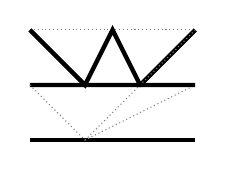
\begin{tikzpicture}[scale=.7,baseline=-5]
\draw[gray,-,thin,densely dotted] (0,1) -- (3,1);%s3t3
\draw[-,ultra thick] (0,0) -- (2,0) -- (3,1);%s2t2
\draw[-,ultra thick] (0,-1) -- (3,-1);%s1t1
\draw[gray,-,thin,densely dotted] (0,0) -- (1,-1) -- (3,0);%s2v1t2
\draw[gray,-,thin,densely dotted] (1,-1) -- (3,1);%v1t3
\draw[-,ultra thick] (0,1) -- (1,0) -- (1.5,1) -- (2,0) -- (3,0);%s3v2
%  \node at (1.5,.3) {$_{(2)}$};  
\end{tikzpicture}\,,
%&
\qquad
K_2 %&
=
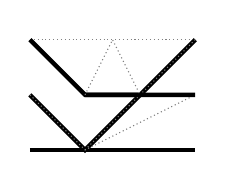
\begin{tikzpicture}[scale=.7,baseline=-5]
\draw[gray,-,thin,densely dotted] (0,1) -- (3,1);%s3t3
\draw[-,ultra thick] (1,0) -- (2,0) -- (3,1);%s2t2
\draw[-,ultra thick] (0,0) -- (1,-1) -- (2,0);
\draw[-,ultra thick] (0,-1) -- (3,-1);%s1t1
\draw[gray,-,thin,densely dotted] (0,0) -- (1,-1) -- (3,0);%s2v1t2
\draw[gray,-,thin,densely dotted] (1,-1) -- (3,1);%v1t3
\draw[-,ultra thick] (0,1) -- (1,0) -- (3,0);%s3v2
\draw[gray,-,thin,densely dotted] (1,0) -- (1.5,1) -- (2,0);
%\node at (1.5,.3) {$_{(2)}$};
\node at (1.5,-.8) {$\phantom{(2)}$};
\node at (1.5,.8) {$\phantom{(2)}$};  
\end{tikzpicture}\,,
%&
\qquad
K_3
%&
=
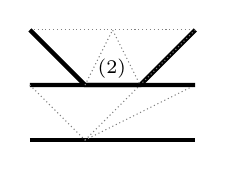
\begin{tikzpicture}[scale=.7,baseline=-5]
\draw[gray,-,thin,densely dotted] (0,1) -- (3,1);%s3t3
\draw[-,ultra thick] (0,0) -- (2,0) -- (3,1);%s2t2
\draw[-,ultra thick] (0,-1) -- (3,-1);%s1t1
\draw[gray,-,thin,densely dotted] (0,0) -- (1,-1) -- (3,0);%s2v1t2
\draw[gray,-,thin,densely dotted] (1,-1) -- (3,1);%v1t3
\draw[-,ultra thick] (0,1) -- (1,0) -- (3,0);%s3v2
\draw[gray,-,thin,densely dotted] (1,0) -- (1.5,1) -- (2,0);
\node at (1.5,.3) {$_{(2)}$};  
\end{tikzpicture}\,,
%\\
%&&&&&\\
%&~\wgt(K_1) = X_1, &\qquad
%&~\wgt(K_2) = X_2, &\qquad
%&~\wgt(K_3) = X_3,
%\end{alignedat}
%\phantom{\right)}
\end{equation}
%\vspace{20mm}
  where the marked edge in $K_3$ has
  %$\small{(2)}$ marking a
  multiplicity $2$.
  %edge in $K_3$,
  %having multiplicity $2$.
  The multisets have weights
  $\wgt(K_1) = feh$,
  $\wgt(K_2) = abfh$,
  $\wgt(K_3) = f^2h$.
%  and
The path families $\pi$, $\rho$, $\sigma$, $\tau$ defined by
\begin{equation}\label{eq:4pathfams}
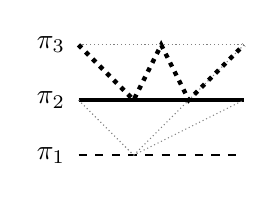
\begin{tikzpicture}[scale=.7,baseline=-5]
\draw[gray,-,thin,densely dotted] (0,1) -- (3,1);%s3t3
\draw[-,ultra thick] (0,-.0) -- (2,-.0) -- (3,-.0);%s2t2
\draw[-,thick,dashed] (0,-1) -- (3,-1);%s1t1
\draw[gray,-,thin,densely dotted] (0,0) -- (1,-1) -- (3,0);%s2v1t2
\draw[gray,-,thin,densely dotted] (1,-1) -- (3,1);%v1t3
%\draw[gray,-,thin,densely dotted] (0,1) -- (1,0);%s3v2
\draw[-,ultra thick, dotted] (0,1) -- (1,0) -- (1.5,1) -- (2,0) -- (3,1);%s3v2
  \node at (-.5,1) {$\pi_3$};  
  \node at (-.5,0) {$\pi_2$};  
  \node at (-.5,-1) {$\pi_1$};  
\end{tikzpicture}\,,
\qquad
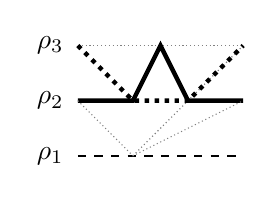
\begin{tikzpicture}[scale=.7,baseline=-5]
\draw[gray,-,thin,densely dotted] (0,1) -- (3,1);%s3t3
\draw[-,ultra thick] (0,-.0) -- (1,-0.0) -- (1.5,1) -- (2,-0.0) -- (3,-.0);%s2t2
\draw[-,thick,dashed] (0,-1) -- (3,-1);%s1t1
\draw[gray,-,thin,densely dotted] (0,0) -- (1,-1) -- (3,0);%s2v1t2
\draw[gray,-,thin,densely dotted] (1,-1) -- (3,1);%v1t3
%\draw[gray,-,thin,densely dotted] (0,1) -- (1,0);%s3v2
\draw[-,ultra thick, dotted] (0,1) -- (1,0.0) -- (2,0.0) -- (3,1);%s3v2
  \node at (-.5,1) {$\rho_3$};  
  \node at (-.5,0) {$\rho_2$};  
  \node at (-.5,-1) {$\rho_1$};  
\end{tikzpicture}\,,
\qquad
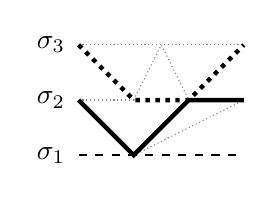
\begin{tikzpicture}[scale=.7,baseline=-5]
\draw[gray,-,thin,densely dotted] (0,1) -- (3,1);%s3t3
\draw[gray,-,thin,densely dotted] (0,0) -- (1,0);%s2v2
\draw[-,thick,dashed] (0,-1) -- (3,-1);%s1t1
\draw[gray,-,thin,densely dotted] (0,0) -- (1,-1) -- (3,0);%s2v1t2
%\draw[-,ultra thick] (0,0) -- (1,-1) -- (3,0);%s2v1
\draw[-,ultra thick] (0,0) -- (1,-1) -- (2,0) -- (3,0);%s2v1t3
\draw[-,ultra thick, dotted] (0,1) -- (1,0) -- (2,0) -- (3,1);%s3v2
\draw[gray,-,thin,densely dotted] (1,0) -- (1.5,1) -- (2,0);
  \node at (-.5,1) {$\sigma_3$};  
  \node at (-.5,0) {$\sigma_2$};  
  \node at (-.5,-1) {$\sigma_1$};  
\end{tikzpicture}\,,
\qquad
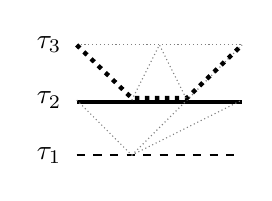
\begin{tikzpicture}[scale=.7,baseline=-5]
\draw[gray,-,thin,densely dotted] (0,1) -- (3,1);%s3t3
\draw[-,ultra thick] (0,-.035) -- (2,-.035) -- (3,-0.035);%s2t2
\draw[-,thick,dashed] (0,-1) -- (3,-1);%s1t1
\draw[gray,-,thin,densely dotted] (0,0) -- (1,-1) -- (3,0);%s2v1t2
\draw[gray,-,thin,densely dotted] (1,-1) -- (3,1);%v1t3
%\draw[gray,-,thin,densely dotted] (0,1) -- (1,0);%s3v2
\draw[-,ultra thick, dotted] (0,1) -- (1,0.035) -- (2,0.035) -- (3,1);%s3v2
\draw[gray,-,thin,densely dotted] (1,0) -- (1.5,1) -- (2,0);
  \node at (-.5,1) {$\tau_3$};  
  \node at (-.5,0) {$\tau_2$};  
  \node at (-.5,-1) {$\tau_1$};  
\end{tikzpicture}
%\,,
%\quad \,
%P(\pi) = \ntnsp
%\begin{tikzpicture}[scale=.7,baseline=-5]
%\draw[fill] (.8,.5) circle (1mm); \node at (.8,1) {$\pi_3$};
%\draw[fill] (.8,-.5) circle (1mm); \node at (.8,-1) {$\pi_1$};
%\draw[fill] (1.6,0) circle (1mm); \node at (1.6,-.5) {$\pi_2$};
%\draw[-,thick] (0,.5) -- (0,-.5);%41
%\draw[-,thick] (.8,.5) -- (0,-.5);%51
%\draw[-,thick] (.8,.5) -- (.8,-.5);%52
%\end{tikzpicture}\ntksp,
%\qquad \qquad
%\quad \,
%\qquad
\end{equation}
satisfy $\Pi_e(K_1) = \{ \pi, \rho \}$,
$\Pi_e(K_2) = \{ \sigma \}$,
$\Pi_e(K_3) = \{ \tau \}$,
and have posets
\begin{equation*}
P(\pi) = \ntksp
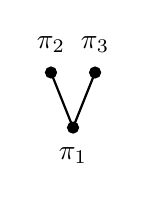
\begin{tikzpicture}[scale=.7,baseline=-5]
\draw[fill] (0,.5) circle (1mm); \node at (0,1) {$\pi_2$};
%\draw[fill] (0,0) circle (1mm); \node at (-.5,0) {$3$};
\draw[fill] (.4,-.5) circle (1mm); \node at (.4,-1) {$\pi_1$};
\draw[fill] (.8,.5) circle (1mm); \node at (.8,1) {$\pi_3$};
%\draw[fill] (.8,-.5) circle (1mm); \node at (.8,-1) {$2$};
%\draw[fill] (1.6,0) circle (1mm); \node at (1.6,-.5) {$3$};
\draw[-,thick] (0,.5) -- (.4,-.5);%41
\draw[-,thick] (.8,.5) -- (.4,-.5);%51
%\draw[-,thick] (.8,.5) -- (.8,-.5);%52
\end{tikzpicture}\ntksp,
\qquad
P(\rho) = \ntksp
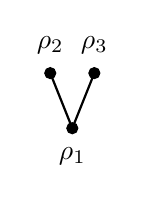
\begin{tikzpicture}[scale=.7,baseline=-5]
\draw[fill] (0,.5) circle (1mm); \node at (0,1) {$\rho_2$};
%\draw[fill] (0,0) circle (1mm); \node at (-.5,0) {$3$};
\draw[fill] (.4,-.5) circle (1mm); \node at (.4,-1) {$\rho_1$};
\draw[fill] (.8,.5) circle (1mm); \node at (.8,1) {$\rho_3$};
%\draw[fill] (.8,-.5) circle (1mm); \node at (.8,-1) {$2$};
%\draw[fill] (1.6,0) circle (1mm); \node at (1.6,-.5) {$3$};
\draw[-,thick] (0,.5) -- (.4,-.5);%41
\draw[-,thick] (.8,.5) -- (.4,-.5);%51
%\draw[-,thick] (.8,.5) -- (.8,-.5);%52
\end{tikzpicture}\ntksp,
\qquad
P(\sigma) = \ntnsp
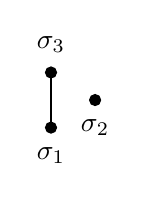
\begin{tikzpicture}[scale=.7,baseline=-5]
\draw[fill] (.8,.5) circle (1mm); \node at (.8,1) {$\sigma_3$};
\draw[fill] (.8,-.5) circle (1mm); \node at (.8,-1) {$\sigma_1$};
\draw[fill] (1.6,0) circle (1mm); \node at (1.6,-.5) {$\sigma_2$};
%\draw[-,thick] (0,.5) -- (0,-.5);%41
%\draw[-,thick] (.8,.5) -- (0,-.5);%51
\draw[-,thick] (.8,.5) -- (.8,-.5);%52
\end{tikzpicture}\ntksp,
\qquad 
P(\tau) = \ntksp
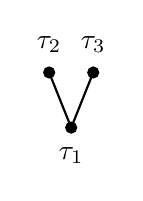
\begin{tikzpicture}[scale=.7,baseline=-5]
\draw[fill] (0,.5) circle (1mm); \node at (0,1) {$\tau_2$};
%\draw[fill] (0,0) circle (1mm); \node at (-.5,0) {$3$};
\draw[fill] (.4,-.5) circle (1mm); \node at (.4,-1) {$\tau_1$};
\draw[fill] (.8,.5) circle (1mm); \node at (.8,1) {$\tau_3$};
%\draw[fill] (.8,-.5) circle (1mm); \node at (.8,-1) {$2$};
%\draw[fill] (1.6,0) circle (1mm); \node at (1.6,-.5) {$3$};
\draw[-,thick] (0,.5) -- (.4,-.5);%41
\draw[-,thick] (.8,.5) -- (.4,-.5);%51
%\draw[-,thick] (.8,.5) -- (.8,-.5);%52
\end{tikzpicture}\ntksp.
%\qquad
\end{equation*}
The standard $F$-tableaux
\begin{equation*}
  \tableau[scY]{\pi_3|\pi_1,\pi_2}\,,\qquad
  \tableau[scY]{\rho_3|\rho_1,\rho_2}\,,\qquad
  \tableau[scY]{\sigma_3|\sigma_1,\sigma_2}\,,\qquad
  \tableau[scY]{\tau_3|\tau_1,\tau_2}  
\end{equation*}
have weights $feh$, $feh$, $abfh$, $f^2e$, respectively.


For an $n \times n$ totally nonnegative matrix $A$
and a trace $\theta \in \trspace n$, 
we may compute $\imm \theta(A)$ by considering
a planar network $F$ having path matrix $A$,
the union over bijective skeletons $K$ of
%each bijective skeleton $K$ of edges of $F$,
%which form bijective skeleta of
%all
path families $\pi \in \Pi_e(K)$,
%$ in $F$,
%each path family $\pi$ of type $e$ in $D$,
%expansions of the
and the corresponding
chromatic symmetric functions $X_{\inc(P(\pi))}$.
Specifically, we have the following~\cite[Cor.\,4.6]{SkanCCS}.
%for each path family $\pi$
%in $F$
\begin{prop}\label{p:immincP}
  For $F$ a planar network having path matrix $A$ and $\theta \in \trspace n$,
  we have
\begin{equation}\label{eq:propcorcomb}
  \imm{\theta}(A) = \sum_K \wgt(K)
  \nTksp \ntnsp \sum_{\pi \in \Pi_e(K)} \nTksp \theta(\inc(P(\pi))),
\end{equation}
where $K$ varies over all bijective skeletons in $F$.  If
for all posets $P$, $\theta(\inc(P))$ counts $P$-tableaux
having a particular property,
%in a subset $\mathcal S$,
then we have
\begin{equation}\label{eq:propcorcomb2}
  \imm{\theta}(A) = \sum_U \wgt(U),
%  \nTksp \ntnsp \sum_{\pi \in \Pi_e(K)} \nTksp \theta(\inc(P(\pi))),
\end{equation}
where the sum is over $F$-tableaux $U$ having the property.
%$\mathcal S$ is
\end{prop}
Proposition~\ref{p:immincP}
has the following consequence~\cite[Cor.\,4.7]{SkanCCS}.
%We also have the following implication.
%(See, e.g., \cite[Cor.\,4.7]{SkanCCS}.)
\begin{cor}\label{c:immincP}
  If $\theta \in \trspace n$ satisfies
  $\theta(\inc(P)) \geq 0$ for all posets $P$, then
  %it also satisfies
the polynomial $\imm\theta(x)$ is totally nonnegative.
\end{cor}

%Proposition~\ref{p:immincP} implies that whenever $\theta(\inc(P))$
%has a combinatorial interpretation for all $P$,
%then so does $\imm{\theta}(A)$ for all totally nonnegative $A$.
%for all totally nonnegative matrices $A$.
By Theorems~\ref{t:epsilonevals} -- \ref{t:KaliGash},
Corollary~\ref{c:immincP} applies to
%this is the case for
induced sign character immanants,
induced trivial character immanants,
and irreducible character immanants indexed by hook partitions.
It does not apply to
%is not the case for
irreducible character immanants in general, because we have
$\chi^\lambda(\inc(P)) < 0$ for some $\lambda$, $P$.
%\begin{cor}\label{c:imminterps}
%  For $\lambda \vdash n$, the polynomials $\imm{\epsilon^\lambda}(x)$
%  and $\imm{\eta^\lambda}(x)$ are totally nonnegative;
%  for $k \leq n$,
%  the polynomial $\imm{\chi^{k1^{n-k}}}(x)$ is totally nonnegative.
%(see, e.g., \cite{SkanCCS} $\star$ better: propositions from the chromatic
%symmetric function section), but
%It is not true for irreducible character immanants in general.
%can be combinatorially
\begin{thm}\label{t:hookimm}
  %For $A$ the path matrix of planar network $D$ of order $n$ and
  For $k \leq n$,
  the polynomial $\imm{\chi^{k1^{n-k}}}(x)$ is totally nonnegative.
    In particular, for $A$ the path matrix of planar network $F$, we have
    \begin{equation*}
      \imm{\chi^{k1^{n-k}}}(A) = \sum_U \wgt(U),
    \end{equation*}
    where the sum is over all standard $F$-tableaux of shape $k1^{n-k}$.
\end{thm}
\bp\label{p:stemimm}
Combinatorially interpret the numbers $\imm{\chi^\lambda}(A)$ in
Theorem~\ref{t:stemimm}.
\ep
%Finding a combinatorial
%interpretation for the number $\imm{\chi^\lambda}(A)$ remains an open problem.
%By
%Proposition~\ref{p:Kali}
%Theorem~\ref{t:KaliGash}
%we do have a combinatorial interpretation in the special case that $\lambda$ is a hook shape.
%($\star$ Define $F$-tableaux earlier, or rewrite this.)

%  we have
%  \begin{equation}\label{eq:hookimm}
%    \imm{\chi^{k1^{n-k}}}(A) = \nTksp \sum_{\pi \in \mcp_e(D)} \nTksp \wgt(\pi)\,
%    (\# \text{ standard $P(\pi)$-tableaux of shape $k1^{n-k}$}).
%  \end{equation}
%  In particular, when $k=n$, we obtain
%  (\ref{eq:introdes}).
%\end{thm}


%For the convenience of the reader we summarize this
%and other known implications as follows.
%($\star$ Keep or cut this?)
%\begin{cor}\label{c:tnnimplications}
%  For $\theta \in \trspace n$, the statements
%  \begin{enumerate}
%  \item $\theta( \wtc w1) \geq 0$ for all permutations $w \in \sn$,
%  \item $\theta( \wtc{w^{(1)}}1 \cdots \wtc{w^{(k)}}1) \geq 0$ for all sequences
%   $(w^{(1)},\dotsc,w^{(k)})$ of maximal elements of parabolic subgroups of $\sn$,
%  \item $\theta(\inc(P)) \geq 0$ for all posets $P$,
%  \item $\imm\theta(A) \geq 0$ for all totally nonnegative matrices $A$,
%  \item $\theta(\inc(P)) \geq 0$ for all
%    unit interval orders $P$,
%  \item $\theta(\inc(P)) \geq 0$ for all
%    $(\mathbf3 + \mathbf1)$-free posets $P$,
%  \item $\theta(\wtc w1) \geq 0$ for all $312$-avoiding permutations $w \in \sn$,
%  \item $\theta(\wtc w1) \geq 0$ for all \pavoiding permutations $w \in \sn$
%\end{enumerate}
%  satisfy the implications (1) $\Rightarrow$ (2) $\Rightarrow$ (4)
%  $\Rightarrow$ (5) $\Leftrightarrow$ (6) $\Leftrightarrow$ (7) $\Leftrightarrow$ (8), and
%  (3) $\Rightarrow$ (4).
%\end{cor}

%\ssec{Monomial immanants}

Corollary~\ref{c:immincP} also does not apply to monomial traces,
which satisfy $\phi^\lambda(\inc(P)) < 0$ for some $\lambda$, $P$.
Nevertheless, Stembridge conjectured that monomial trace immanants are totally
nonnegative~\cite[Conj.\,2.1]{StemConj}.
\begin{conj}\label{c:monimm}
  For $\lambda \vdash n$ the polynomial $\imm{\phi^\lambda}(x)$ is totally
  nonnegative.
  %and $A$ totally nonnegative we have
  %$\imm{\phi^\lambda}(A) \geq 0$.
\end{conj}

%When $A$ is the antiadjacency matrix of a unit interval order,
%the above formula simplifies significantly~\cite[Eqn.\,(3.5)]{CHSSkanEKL}.
%\begin{cor}
%  For $A$ the antiadjacency matrix of a unit interval order $P$
%  labeled as in Algorithm~\ref{a:PtoC}, we have
%\begin{equation}\label{eq:propcorcomb}
%  \imm{\theta}(A) = \theta(\inc(P)).
%\end{equation}
%\end{cor}
%\begin{proof}
%  Let $w$ be the permutation associated by Algorithm~\ref{a:PtoC} to $P$.
%  By ($\star$ cite this) we have
%  \begin{equation*}
%    \permmon av = \begin{cases} 1 &\text{if $v \leq w$},\\
%                                0 &\text{otherwise}.
%                  \end{cases}
%    \end{equation*}
%  Thus we can
%  write
%  \begin{equation*}
%    \imm{\theta}(A) =
%    \sum_{v \in \sn} \theta(v) \permmon av
%    = \sum_{v \leq w} \theta(v) 
%    = \theta \Big( \sum_{v \leq w} v \Big) = \theta(C'_w(1)).
%  \end{equation*}
%  By Observation~\ref{o:yyx} and Proposition~\ref{p:uioto312avoid},
%  this is $\theta(\inc(P))$.
%\end{proof}

Some evidence for Conjecture~\ref{c:monimm} follows from recent work
of Hikita~\cite{HikitaProof}.
%Hikita proved a weaker statement. ($\star$ Cite.)
%($\star$ Include this?)
\begin{prop}
  If $A$ is the antiadjacency matrix of a unit interval order
  labeled as in Step 2 of Algorithm~\ref{a:PtoC},
%  (path matrix of a descending star network?)
  then for all $\lambda \vdash n$ we have that $\imm{\phi^\lambda}(A) \geq 0$.
\end{prop}
\begin{proof}
  Let $A$ be the antiadjacency matrix of unit interval order $P$,
  labeled as in Step 2 of Algorithm~\ref{a:PtoC},
  and let $w$ be the $312$-avoiding permutation
  associated to $P$ by Step 3 of Algorithm~\ref{a:PtoC}.
  It is well known that the entries of $A$ which are equal to $1$
  form a Ferrers shape, and that we have
  \begin{equation*}
    \permmon av = \begin{cases} 1 &\text{if $v \leq w$},\\
      0 &\text{otherwise}.
    \end{cases}
  \end{equation*}
  (See, e.g., \cite[Prop.\,19, Prop.\,22]{WatsonBruhat}.)  Thus we have
  \begin{equation*}
    \imm{\phi^\lambda}(A) =
    \sum_{v \in \sn} \phi^\lambda(v) \permmon av
    = \sum_{v \leq w} \phi^\lambda(v) 
    = \phi^\lambda \Big( \sum_{v \leq w} v \Big)
    = \phi^\lambda(C'_w(1)).
  \end{equation*}
  By Proposition~\ref{p:uioto312avoid} this number is $\phi^\lambda(\inc(P))$,
%  \end{equation*}
  and by Theorem~\ref{t:hikita} it is nonnegative.
\end{proof}
%\begin{proof}
%  (Original proof)  
%  Decomposing $P$ as
%  $P = P_1 \oplus \cdots \oplus P_r$~\cite[\S 3.2]{StanEC1},
%  as finely as possible
%  so that all elements of $P_i$ are less than all elements of $P_{i+1}$
%  for $i = 1,\dotsc,r-1$,
%  we see that $A$ has a lower triangular block decomposition of the form
%  $A = (A_{i,j})_{i,j=1}^r$
%  in which $A_{i,i}$ is the antiadjacency matrix of $P_{i,i}$
%  for $i = 1,\dotsc,r$,
%  and $A_{i,j}$ is a matrix of all ones whenever $i > j$.
%
%  Let $w$ be the $312$-avoiding permutation
%  associated to $P$ by Step 3 of Algorithm~\ref{a:PtoC}.
%  A factorization of $w$ called the {\em zig-zag factorization}
%  in \cite[\S 3]{SkanNNDCB}
%  associates to $w$ a planar network $F_w$
%  called a {\em zig-zag network}
%  in \cite[\S 5]{SkanNNDCB}, and more specifically,
%  a {\em descending star network} in \cite[\S 3]{CHSSkanEKL}.
%  All edge weights of $F_w$ are $1$.
%  By \cite[Lem.\,5.3\,(1)]{SkanNNDCB},
%  the unique bijective skeleton in $F_w$ is $F_w$ itself,
%  by \cite[Lem.\,5.3\,(3)]{SkanNNDCB},
%  the set $\Pi_e(F_w)$ consists of a unique path family $\pi$
%  and by \cite[Thm.\,4.1]{CHSSkanEKL},
%  the poset $P(\pi)$ is precisely the unit interval order $P$.
%  It is straightforward to show that the path matrix of
%  $F_w$ is the $0$-$1$ block-diagonal matrix
%  $B = A_{1,1}
%  \oplus \cdots \oplus A_{r,r}$.
%  Thus for all $v \in \sn$, the matrices $A$, $B$
%  satisfy
%  \begin{equation*}
%    \permmon av = \permmon bv,
%  \end{equation*}
%  and for all $\theta \in \trspace n$ we have
%  $\imm{\theta}(A) = \imm{\theta}(B)$.
%  In particular by (\ref{eq:propcorcomb})
%  we have
%  for all $\lambda \vdash n$ that
%    $\imm{\phi^\lambda}(A) = \imm{\phi^\lambda}(B) = \phi^\lambda(\inc(P))$.
%  By Theorem~\ref{t:hikita}, this is nonnegative.
%  \end{proof}

More evidence for Conjecture~\ref{c:monimm} follows from
%weaker statement follows from
work of Stanley~\cite{StanSymm}.  
\begin{prop}\label{p:sumofmonimms}
  For $\ell = 1,\dotsc,n$, the sum
    \begin{equation}\label{eq:sumofmux}
        \sumsb{\mu \vdash n\\\ell(\mu) = \ell} \ntnsp \imm{\phi^\mu}(x)
    \end{equation}
    of monomial immanants is a totally nonnegative polynomial.
    In particular, for $A$ the path matrix of planar network $F$, we have
    \begin{equation}\label{eq:sumofmuA}
      \sumsb{\mu \vdash n\\\ell(\mu) = \ell} \ntnsp \imm{\phi^\mu}(A) =
      \sum_U \wgt(U), 
    \end{equation}
    where the sum is over row-semistrict $F$-tableaux $U$
    of shape $n$ having $\ell$ records.
\end{prop}
\begin{proof}
  %Fix $\ell$ and
  Fix a totally nonnegative matrix $A$
  and
 define the trace
  \begin{equation}%\label{eq:thetaldef}
    \theta^\ell = \sumsb{\mu \vdash n\\\ell(\mu) = \ell} \ntnsp \phi^\mu
  \end{equation}
  so that the left-hand side of (\ref{eq:sumofmuA}) is $\imm{\theta^\ell}(A)$.
  By
  %Theorem~\ref{t:tnnconv} $A$
  %is the path matrix of some planar network $F$ and 
  %by
  Proposition~\ref{p:immincP}
  %this is
  we have that
  \begin{equation*}
    \imm{\theta^\ell}(A) =
    \sum_K \wgt(K) \nTksp
    \sum_{\pi \in \Pi_e(K)} \nTksp \theta^\ell(\inc(P(\pi)),
%    \theta(z(K))
%    = \sum_K \wgt(K) \theta \Big(\nTksp\sum_{\pi \in \Pi_e(K)} \nTksp \type(w)\Big),
  \end{equation*}
  where the first sum is over all bijective skeletons $K$ in $F$.
  By Proposition~\ref{p:stanksources}, the inner sum equals the
  number of
%  $P(\pi)$-descent-free $P(\pi)$-permutations
  descent-free $P(\pi)$-tableaux of shape $n$
  having $\ell$
  %$P(\pi)$-records.
  records.
  %But each $P(\pi)$-descent-free $P(\pi)$-permutation
  Equivalently, it equals the number of
  row-semistrict $F$-tableaux of shape $n$ having $\ell$
  %$P(\pi)$-records.
  records.
  Thus the evaluation (\ref{eq:sumofmuA}) has the desired interpretation.
  Since each such $F$-tableau has weight
  %of that $F$-tableau is
  $\wgt(K) \geq 0$, 
  the polynomial (\ref{eq:sumofmux}) is totally nonnegative.  
%  ($\star$ Explain how this comes from Stanley's result.)
\end{proof}
For example, let $F$, $A$ be as in (\ref{eq:planarnet}).
The path families $\pi$, $\rho$, $\sigma$, and $\tau$
in (\ref{eq:4pathfams}) contribute $7$ to $\imm{\theta^2}(A)$,
with each of the tableaux
%Circling records, we have
\begin{equation*}
\tableau[scY]{\pi_1,\pi_2,\pi_3}\,, \quad
\tableau[scY]{\pi_1,\pi_3,\pi_2}\,, \quad
\tableau[scY]{\rho_1,\rho_2,\rho_3}\,, \quad
\tableau[scY]{\rho_1,\rho_3,\rho_2}\,, \quad
\tableau[scY]{\sigma_1,\sigma_3,\sigma_2}\,, \quad
\tableau[scY]{\tau_1,\tau_2,\tau_3}\,, \quad
\tableau[scY]{\tau_1,\tau_3,\tau_2}
\end{equation*}
having records in positions $1$ and $2$.
%($\star$ Include an example?)

\section{Main result and open problems}\label{s:main}

We now show that Heyfron's inequalities (Theorem~\ref{t:heyfron})
%(\ref{eq:heyfron})
hold not only for Hermitian positive semidefinite matrices,
but also for totally nonnegative matrices.

\begin{thm}\label{t:main}
  For each $n \times n$ totally nonnegative matrix $A$ we have
\begin{equation*}
   \perm(A)=\frac{\imm{\chi^n}(A)}{\chi^{n}(e)}\geq \frac{\imm{\chi^{n-1,1}}(A)}{\chi^{n-1,1}(e)}\geq \frac{\imm{\chi^{ n-2,1,1}}(A)}{\chi^{n-2,1,1}(e)}\geq \cdots \geq \frac{\imm{\chi^{1,\dotsc,1}}(A)}{\chi^{1,\dotsc,1}(e)}=\det(A).
\end{equation*} 
Equivalently, for $k = 2,\dotsc,n$,
the difference
        \begin{equation}\label{eq:thediff}
        \frac{\imm{\chi^{k1^{n-k}}}(x)}{\chi^{k1^{n-k}}(e)}
        -
        \frac{\imm{\chi^{(k-1)1^{n-k+1}}}(x)}{\chi^{(k-1)1^{n-k+1}}(e)}
        =
         \frac{\imm{\chi^{k1^{n-k}}}(x)}{\binom{n-1}{k-1}}
        -
        \frac{\imm{\chi^{(k-1)1^{n-k+1}}}(x)}{\binom{n-1}{k-2}}
    \end{equation}
        is a totally nonnegative polynomial.
\end{thm}
\begin{proof}[First proof]
%  The derired inequalities hold if and only if
%  the difference
        Multiplying (\ref{eq:thediff}) by $\tfrac{(n-1)!}{(n-k)!(k-2)!}$,
        we have
%        This in turn is equivalent to the nonnegativity of
        \begin{equation}\label{eq:theseconddiff}
          (k-1)\imm{\chi^{k1^{n-k}}}(x) - (n-k+1)\imm{\chi^{(k-1)1^{n-k+1}}}(x).
        \end{equation}
        Let $A$ be an $n \times n$ totally nonnegative matrix.
        By Theorem~\ref{t:tnnconv}, we may choose a planar network $F$
        whose path matrix is $A$.
        By Theorem~\ref{t:hookimm},
        the evaluation of (\ref{eq:theseconddiff}) at $A$ equals
        \begin{equation}\label{eq:eval}
          \begin{aligned}
%          &(k-1) \nTksp \sum_{\pi \in \Pi_e(F)}\nTksp \wgt(\pi) d_k(\pi) -
%          (n-k+1) \nTksp \sum_{\pi \in \Pi_e(F)} \nTksp \wgt(\pi) d_{k-1}(\pi)\\
%            &= \nTksp \sum_{\pi \in \Pi_e(F)} \nTksp
%            \wgt(\pi) [(k-1)d_k(\pi) - (n-k+1)d_{k-1}(\pi)],
          &(k-1) \ntnsp \sum_\pi \wgt(\pi) d_k(\pi) -
          (n-k+1) \ntnsp \sum_\pi \wgt(\pi) d_{k-1}(\pi)\\
            &= \sum_\pi \wgt(\pi) [(k-1)d_k(\pi) - (n-k+1)d_{k-1}(\pi)],
          \end{aligned}
        \end{equation}
        where $d_k(\pi)$ is the number of standard $\pi$-tableaux
        of shape $k 1^{n-k}$, and
        the sums are over
        \begin{equation*}
          \pi \in \bigcup_K
          %{\substack{K \text{a}\\\text{bijective}\\{\text{skeleton}\\\text{in} F}}}
          \Pi_e(K)
        \end{equation*}
        with $K$ varying over all bijective skeletons in $F$.
        By Proposition~\ref{l:hookineq}
        %and its proof,
        the difference in square brackets in the last sum equals
        the number of standard $P(\pi)$-tableaux
        of shape $k1^{n-k}$ with one marked
        entry in columns $2,\dotsc,k$ which is incomparable to at
        least one entry in an earlier column.
        %such that this entry ...
        %(or other combinatorial interpretation.)
        %which is nonnegative for each $n$-element poset $P$.
        Since this number and $\wgt(\pi)$ are nonnegative, the evaluation
        (\ref{eq:eval}) is nonnegative.  Thus the polynomial
        (\ref{eq:theseconddiff}) is totally nonnegative
        and so is the polynomial (\ref{eq:thediff}).
\end{proof}
\begin{proof}[Second proof]
  Define the traces $\theta^1, \dotsc, \theta^n$
  as in (\ref{eq:thetaldef}).
  %Proposition~\ref{p:thetak}.
%  For $k = 1,\dotsc, n$ define the trace
%  \begin{equation*}
%    \theta^k = \sumsb{\mu \vdash n \\\ell(\mu) = \ell} \phi^\mu.
%    \end{equation*}
  By Proposition~\ref{p:hookKostka}
  %Corollary~\ref{c:hookirrmon}, all of
  we have that
  the hook irreducible character immanant indexed by $k1^{n-k}$
  belongs to the $n$-dimensional space spanned by
  $\imm{\theta^1}(x), \dotsc, \imm{\theta^n}(x)$.  Specifically,
  %$\imm{\chi^{k1^{n-k}}}(x)$
%  satisfies
    \begin{equation}\label{eq:hookirrmon}
      \imm{\chi^{k1^{n-k}}}(x) =
      \nTksp \sum_{\ell = n-k+1}^n \ntksp \binom{\ell-1}{n-k} \, \imm{\theta^\ell}(x).
      %\sumsb{\mu \vdash n\\\ell(\mu) = \ell} \ntnsp \imm{\phi^\mu}(x).
    \end{equation}
%    for $k = 1,\dotsc,n$
    %and t
%    Therefore it 
%    \begin{equation}\label{eq:monsumbasis}     
%      \bigg\{ M_\ell(x) \defeq \sumsb{\mu \vdash n\\ \ntksp \ell(\mu) = \ell}
%      \imm{\phi^\mu}(x) \,\bigg|\, \ell = 1,\dotsc, n \bigg\}.
%    \end{equation}
It follows that for $k = 2,\dotsc,n$, the difference (\ref{eq:thediff})
      expands in the basis of $\theta^\ell$-immanants as
      %equals
      %expands in the basis (\ref{eq:monsumbasis}) as
      $c_{k,1} \imm{\theta^1}(x) + \cdots + c_{k,n} \imm{\theta^n}(x)$
%      \begin{equation*}
%        \sum_{\ell = 1}^n c_{k,\ell}
%        \ntksp \sumsb{\mu \vdash n\\\ell(\mu) = \ell} \ntksp \imm{\phi^\mu}(x),
%        \end{equation*}
    with nonnegative coefficients
    \begin{equation*}
        c_{k,\ell} = \frac{\binom{\ell-1}{n-k}}{\binom{n-1}{k-1}} - \frac{\binom{\ell-1}{n-k+1}}{\binom{n-1}{k-2}} = 
        \begin{cases}
        0
%        \overset {\phantom a}0\phantom{\frac1{\binom nk}}
        &\text{if $\ell = 1,\dotsc,n-k$},\\
            \text{\raisebox{1.25mm}{$\frac{1}{\binom{n-1}{k-1}}$}} &\text{if $\ell = n-k+1$},\\
            \frac{n-\ell}{\ell-(n-k+1)} &\text{if $\ell = n-k+2, \dotsc, n$}.
        \end{cases}
    \end{equation*}
    % \begin{equation*}
    %     \frac{1}{\tbinom{n-1}{k-1}} \nTksp \nTksp \nTksp \sumsb{\mu \vdash n\\\phantom{Mv}\ell(\mu) = n-k+1}\nTksp \nTksp \nTksp \imm{\phi^{\mu}}(x)
    %     + \nTksp \nTksp \ntksp \sum_{\phantom{Mv}\ell = n-k+2}^n
    %     \tfrac{n-\ell}{\ell-(n-k+1)} \sumsb{\mu \vdash n\\ \ell(\mu) = \ell} \imm{\phi^\mu}(x).
    % \end{equation*}
    %\end{enumerate}
    By Proposition~\ref{p:sumofmonimms}, each immanant $\imm{\theta^\ell}(x)$
    %element of the basis (\ref{eq:monsumbasis})
    is a totally nonnegative polynomial.
    Thus for $k = 2,\dotsc, n$
    the difference (\ref{eq:thediff}) is as well.
    %, and we have
    %\begin{equation*}
    %          \frac{\imm{\chi^{k1^{n-k}}}(A)}{\chi^{k1^{n-k}}(e)}
    %    \geq
    %    \frac{\imm{\chi^{(k-1)1^{n-k+1}}}(A)}{\chi^{(k-1)1^{n-k+1}}(e)}
    %\end{equation*}
    %for all $n \times n$ totally nonnegative matrices $A$.
\end{proof}
Theorem~\ref{t:main} thus provides some progress on the problem
of understanding (\ref{eq:irrimmineq}).
\bp
Characterization the pairs $(\lambda,\mu)$
of partitions satisfying
\begin{equation}\label{eq:irrimmineq2}
  \frac{\imm{\chi^\lambda}(A)}{\chi^\lambda(e)}
  \geq
  \frac{\imm{\chi^\mu}(A)}{\chi^\mu(e)}
\end{equation}
%(\ref{irrimmineq})
for all totally nonnegative
or Hermitian positive semidefinite matrices.
\ep

Generalizing Heyfron's inequalities, Pate~\cite{PatePICIGMF}
proved that if $\lambda$, $\mu$
are two partitions of $n$, with $k$ the
multiplicity of $\lambda_1$ in $\lambda = (\lambda_1,\dotsc,\lambda_\ell)$
and
\begin{equation}\label{eq:pate}
  \mu = (\lambda_1 - 1, \dotsc, \lambda_k - 1,
  \lambda_{k+1}, \dotsc, \lambda_\ell, \;
  \underbrace{\ntksp 1, \dotsc, 1 \ntksp }_k\;),
  \end{equation}
then we have (\ref{eq:irrimmineq2}) for all Hermitian positive semidefinite
matrices.  In other words, the Young diagram of $\mu$ is obtained by
removing the rightmost column of the Young diagram of $\lambda$
and by appending this to the first column, for example
\begin{equation*}
  \lambda =
   (4, 4, 3, 2) =
      \tableau[scY]
        {\ , \ |
         \ , \ , \ |
         \ , \ , \ , \ |
         \ , \ , \ , \ }\,,
      \qquad
      \mu =
   (3, 3, 3, 2, 1, 1) =
      \tableau[scY]
        {\ |
         \ |
         \ , \ |
         \ , \ , \ |
         \ , \ , \ |
         \ , \ , \ }\,.
\end{equation*}
Perhaps this inequality holds
for totally nonnegative matrices as well.
\bp
Decide if Pate's inequality, i.e., (\ref{eq:irrimmineq2}) for $\lambda$, $\mu$
satisfying (\ref{eq:pate}), holds for all totally nonnegative matrices.
\ep

Theorem~\ref{t:main} and its proofs suggest several other open problems.
Haiman~\cite[Conj.\.2.1]{HaimanHecke} has conjectured that
certain $q$-analogs $\phi_q^\lambda$ and $C'_w(q)$
of the monomial trace $\phi^\lambda$
and Kazhdan--Lusztig basis element $C'_w(1)$
satisfy
\begin{equation*}
  %\label{eq:haimanconj}
  \phi_q^\lambda(\qp{\ell(w)}2C'_w(q)) \in \mathbb N[q]
  \end{equation*}
for all $\lambda$ and all $w$.
(See \cite{HaimanHecke} for definitions.)
Perhaps the following weaker statment would be easier to prove.
\bp
Show that for $\ell = 1,\dotsc,n$ and all $w \in \sn$ we have
$\theta_q^\ell(\qp{\ell(w)}2C'_w(q)) \in \mathbb N[q]$,
where
\begin{equation*}
  \theta_q^\ell = \sumsb{\lambda \vdash n\\ \ell(\lambda) = \ell} \phi_q^\lambda.
  \end{equation*}
\ep
\noindent
This is known to be true for $w$ \avoidingp.
(See, e.g., \cite[Thm.\,5.6]{CHSSkanEKL}, \cite[Prop.\,5.4]{SkanCCS}.)

It would also be interesting to find an analog of the
Littlewood--Merris--Watkins identities (\ref{eq:lmw}), (\ref{eq:lmw2})
for the immanants
$\{ \imm{\theta^\ell}(x) \,|\, \ell \in [n] \}$.

\bp For $\ell = 1,\dotsc, n$, find an expression for the
immanant $\imm{\theta^\ell}(x)$ which makes its
%in terms of matrix minors so that its
total nonnegativity apparent.
\ep

%($\star$ Mention also \cite{PatePICIGMF}.
%Is Pate's inequality
%true for TNN matrices also?  Specifically, does one of the proofs
%of the main theorem adapt to Pate's inequality?)

\section{Acknowledgements}

The author is grateful to Alex Fink
and Keith McNulty for helpful conversations,
and to
the Mathematics Genealogy Project
for displaying Keith McNulty's relevant but unpublished thesis.

\bibliography{skan}
\end{document}

